\documentclass[a4paper,14pt]{extreport} %размер бумаги устанавливаем А4, шрифт 14пунктов
\usepackage[T2A]{fontenc}
\usepackage[utf8]{inputenc}
\usepackage[english,russian]{babel}
\usepackage{amssymb,amsfonts,amsmath,enumerate,float} % подключаем нужные пакеты расширений
\usepackage{graphicx} % хотим вставлять в диплом рисунки
\usepackage{longtable} % для таблиц длиннее, чем на страницу
\usepackage{misccorr} % Добавляем "точки" после названий разделов
\usepackage{geometry} % Меняем поля страницы
\usepackage{indentfirst}%отступ первого абзаца после названия главы
\usepackage{setspace}
\usepackage{fancyhdr} 
\usepackage{lastpage}
\usepackage{titlesec} % название главы по центру
\usepackage[nottoc,notlof,notlot]{tocbibind} 
\usepackage[figure,table]{totalcount}
\usepackage{caption}
\captionsetup[figure]{font=small}
\usepackage{etoolbox}

\usepackage{listings} % code snippets
\usepackage{lmodern}  % for bold teletype font
\usepackage{amsmath}  % for \hookrightarrow
\usepackage{xcolor}   % for \textcolor
\usepackage{listings}
\lstset{
  basicstyle=\ttfamily,
  columns=fullflexible,
%   frame=single,
  breaklines=true,
%   postbreak=\mbox{\textcolor{red}{$\hookrightarrow$}\space},
}
% MY LITERATURE REPORT:
\usepackage{csquotes}% Recommended
\bibliographystyle{bibliography/gost-numeric.bbx}
\usepackage[
    parentracker=true,
    backend=biber,
    hyperref=false,
    bibencoding=utf8,
    style=gost-numeric,
    language=auto,
    autolang=other,
    citestyle=gost-numeric,
    defernumbers=true,
    bibstyle=gost-numeric,
    sorting=none,
]{biblatex}
\addbibresource{bibliography/library.bib}
\usepackage{textcomp}
% ^

% fixing biblatex-gost formatting:
\renewcommand{\mkgostheading}{\textrm} % сделать авторов в списке литературы по госту
% ^

\graphicspath{{images/}}



\makeatletter
% \renewcommand{\@biblabel}[1]{#1.} % Заменяем библиографию с квадратных скобок на точку
\makeatother

\geometry{left=2.5cm}% левое поле
\geometry{right=2cm}% правое поле
\geometry{top=2cm}% верхнее поле
\geometry{bottom=2cm}% нижнее поле

\setcounter{secnumdepth}{4}% уровень вложенности счётчиков

\onehalfspacing



\usepackage{titletoc} %

\titleclass{\prettypart}{top}[\part]


\titleformat{\prettypart}
{\normalfont\centering}{}{0pt}{\normalfont}


\titleformat{\part}
{\normalfont\bfseries\centering}{}{0pt}{\normalfont\bfseries}



\titleformat{\chapter}
{\normalfont\bfseries}{\thechapter}{1em}{}

\titleformat{\section}
{\normalfont\bfseries}{\thesection}{1em}{}

\titleformat{\subsection}[block]
{\normalfont\bfseries}{\thesubsection}{1em}{}

\titleformat{\subsubsection}[block]
{\normalfont\bfseries}{\thesubsubsection}{1em}{}




% Настройка вертикальных и горизонтальных отступов
\titlespacing*{\prettypart}{0pt}{*4}{*4}
\titlespacing*{\chapter}{0.75cm}{*4}{*4}
\titlespacing*{\section}{\parindent}{*4}{*4}
\titlespacing*{\subsection}{\parindent}{*4}{*4}

\newcounter{prettypart}
\titlecontents{prettypart}{\vspace{1em}\normalfont}{}{}{\titlerule*[1pc]{.}\normalfont\contentspage}

\titlecontents{part}{\vspace{1em}\normalfont\bfseries}{}{}{\titlerule*[1pc]{.}\normalfont\contentspage}

% to make a "1." before all the chapters, comment this:
% \titlecontents{chapter}{\vspace{1em}\normalfont\bfseries}this!!!->>> {}{}{\titlerule*[1pc]{.}\normalfont\bfseries\contentspage}
% выравнивание всех chapter чтобы был отступ по горизонтали в содержании
\titlecontents{chapter}{
    \hspace*{1em}
    \normalfont
    \bfseries
}{\bfseries \contentslabel{-.1em} \hspace*{1em} }{}{
    \titlerule*[1pc]{.}
    \normalfont
    \bfseries
    \contentspage
}
\titlecontents{section}{
    \hspace*{2em}
}{ \contentslabel{} \hspace*{1em} }{}{
    \titlerule*[1pc]{.}
    \contentspage
}



% нумерация снизу по середине
\pagestyle{fancy} 
\lhead{} \chead{} \rhead{}
\lfoot{} \cfoot{\normalsize\thepage} \rfoot{}
\renewcommand{\headrulewidth}{0pt}
\renewcommand{\footrulewidth}{0pt}
\fancypagestyle{plain}{%
    % \fancyhf{} % clear all header and footer fields
    % \fancyhead[RE,CC]{\normalsize \thepage} % Even page, Odd page; Right, Left, Center
    % тоже снизу по середине:
    % \cfoot{\thepage}
    \renewcommand{\headrulewidth}{0pt}
    \renewcommand{\footrulewidth}{0pt}
}

\makeatletter
\makeatother 

\usepackage[figurename=Рисунок]{caption}
\usepackage[labelsep=space]{caption}
% \counterwithout{figure}{section}
\counterwithout{figure}{subsection}

\usepackage{ragged2e} % for /justify command

\setcounter{tocdepth}{3}


\setlength{\parindent}{1cm}

\newcommand{\quotes}[1]{``#1''}


% to use bold commands (for bold text and etc)
% \renewcommand{\rmdefault}{cmr} % Шрифт с засечками
\renewcommand{\rmdefault}{Tempora-TLF} %tempora font (almost like Times New Roman)
% \renewcommand{\sfdefault}{cmss} % Шрифт без засечек
\renewcommand{\ttdefault}{cmtt} % Моноширинный шрифт

\begin{document}

% \title{Бессерверная система управления цифровыми активами с автоматическим развертыванием в облаке AWS \\(Amazon Web Services).}
\author{Юлдашев Андрей Алишерович}
\maketitle% это титульный лист

\setcounter{page}{2}
\begin{center}
  РЕФЕРАТ
\end{center}

Выпускная квалификационная работа содержит \pageref{LastPage}\ страниц, \totalfigures\ рисунков, 31 источник.


\noindent \justify \sloppy СИСТЕМА УПРАВЛЕНИЯ ЦИФРОВЫМИ АКТИВАМИ, ВЕБ-ПРИЛОЖЕНИЯ, ОБЛАЧНОЕ ХРАНИЛИЩЕ, АВТОМАТИЗИРОВАННОЕ РАЗВОРАЧИВАНИЕ, DEVOPS, ОБЛАЧНЫЕ ТЕХНОЛОГИИ, AMAZON WEB SERVICES, SERVERLESS, NOSQL.


В данной работе поставлена и решена задача создания Системы управления цифровыми активами, использующей облачные технологии, архитектурный подход Serverless и автоматическое разворачивание в облачном провайдере.

В теоретической части работы приведены рассуждения, предшествующие постановке задачи, оценена актуальность задачи и исследованы существующие аналоги.

В практической части работы описан разработанный подход к решению задачи с использованием Serverless подхода, предоставляемого облачными технологиями, а также рассмотрены ключевые элементы DAM"=системы, как именно происходит работа приложения и автоматизированное развертывание в AWS (Amazon Web Services).
\pagebreak

\renewcommand{\contentsname}{\centering \normalfont СОДЕРЖАНИЕ \par} 
% {\renewcommand{\baselinestretch}{1.0}
% \tableofcontents
       
% }
\tableofcontents
\pagebreak

% \addcontentsline{toc}{prettypart}{СПИСОК ТЕРМИНОВ И СОКРАЩЕНИЙ}
\prettypart{ТЕРМИНЫ И ОПРЕДЕЛЕНИЯ}

% \newcolumntype{s}{>{\hsize=.25\hsize \raggedright\arraybackslash}X} \newcolumntype{b}{>{\hsize=.75\hsize}X}

% \begin{tabularx}{\textwidth}{|sb|} { 
%      >{\raggedright\arraybackslash}X 
%      >{\raggedright\arraybackslash}X 
%      >{\raggedright\arraybackslash}X  
%   }

%  API & --- & это набор определений и протоколов для создания и интеграции прикладного программного обеспечения. Иногда это называют контрактом между поставщиком информации и пользователем информации, устанавливающим контент, требуемый от потребителя (запрос), и контент, требуемый производителем (ответ). Например, дизайн API для службы погоды может указывать, что пользователь предоставляет почтовый индекс, а производитель отвечает протоколом, состоящим из двух частей, первая из которых соответствует высокой температуре, а вторая - низкой \\
%  item 21  & item 22  & item 23  \\
% \end{tabularx}


% \noindent
% \begin{tabular}{
%   p{\dimexpr.2\linewidth-2\tabcolsep-1.3333\arrayrulewidth}% column 1
%   p{\dimexpr.1\linewidth-2\tabcolsep-1.3333\arrayrulewidth}% column 2
%   p{\dimexpr.25\linewidth-2\tabcolsep-1.3333\arrayrulewidth}% column 3
%   }
%   \raggedright TERM& --- & asdgasgasgasfgadfgafadf \\
% \end{tabular}





\RaggedRight \noindent \justify \sloppy API
\begin{minipage}[t][][t]{3.15cm}
\RaggedLeft
  ---
\end{minipage}
\begin{minipage}[t][][t]{0.75\textwidth}
\RaggedRight  \justify \sloppy
 это набор определений и протоколов для создания и интеграции прикладного программного обеспечения. Иногда это называют контрактом между поставщиком информации и пользователем информации, устанавливающим контент, требуемый от потребителя (запрос), и контент, требуемый производителем (ответ). Например, дизайн API для службы погоды может указывать, что пользователь предоставляет почтовый индекс, а производитель отвечает протоколом, состоящим из двух частей, первая из которых соответствует высокой температуре, а вторая - низкой \\
\end{minipage}



\RaggedRight \noindent \justify \sloppy Back"=End
\begin{minipage}[t][][t]{1.9cm}
\RaggedLeft
  ---
\end{minipage}
\begin{minipage}[t][][t]{0.75\textwidth}
\RaggedRight  \justify \sloppy
 это серверная часть, та часть приложения, которая скрыта от пользователя. Эта часть отвечает за обработку данных, их хранение и математические операции \\
\end{minipage}


% \begin{minipage}{4cm}
\RaggedRight \noindent \justify \sloppy DAM"=система
% \end{minipage}%
\begin{minipage}[t][][t]{1cm}
\RaggedLeft
  ---
% 123.456.7890
\end{minipage}%
\begin{minipage}[t][][t]{0.75\textwidth}
\RaggedRight  \justify \sloppy
 это программный продукт, предназначенный для управления информацией, используемой в бизнес"=целях. Сортировка, поиск необходимых файлов и структуризация для быстрого и удобного хранения данных, а также менеджмент прав на использование всей этой информацией сотрудниками компании. (DAM"= сокращение от Digital Asset Management) \\
\end{minipage}



\RaggedRight \noindent \justify \sloppy Endpoint
\begin{minipage}[t][][t]{1.9cm}
\RaggedLeft
  ---
\end{minipage}
\begin{minipage}[t][][t]{0.75\textwidth}
\RaggedRight  \justify \sloppy
это одна из рубежных точек канала связи. Когда две системы связываются друг с другом через API, точки взаимодействия и называются endpoints. Для API конечная точка может включать URL-адрес сервера или службы. Каждая конечная точка - это место, из которого API-интерфейсы могут получить доступ к ресурсам, необходимым для выполнения своей функции \\
\end{minipage}



\RaggedRight \noindent \justify \sloppy Front"=End
\begin{minipage}[t][][t]{1.7cm}
\RaggedLeft
  ---
\end{minipage}
\begin{minipage}[t][][t]{0.75\textwidth}
\RaggedRight  \justify \sloppy
это то, что пользователь видит и с чем взаимодействует (пользовательский интерфейс) \\
\end{minipage}



\RaggedRight \noindent GSI и LSI
\begin{minipage}[t][][t]{1.7cm}
\RaggedLeft
  ---
\end{minipage}
\begin{minipage}[t][][t]{0.75\textwidth}
\RaggedRight  \justify \sloppy
это вторичные индексы базы данных AWS DynamoDB. GSI (Global Secondary Index) позволяет выполнять запросы по всей таблице и по всем разделам, меняя основной ключ по которому будет производиться агрегация данных. LSI (Local Secondary Index) позволяет выполнять запросы по одной секции, указанной значением Sort Key в запросе, LSI может быть применен только для изменения вторичного ключа, по которому производиться отбор и сортировка данных, основной ключ поиска (Primary Key) будет совпадать с Primary ключом таблицы \\
\end{minipage}



\RaggedRight \noindent \justify \sloppy Query parameters
\begin{minipage}[t][][t]{0.4cm}
\RaggedLeft
  ---
\end{minipage}
\begin{minipage}[t][][t]{0.75\textwidth}
\RaggedRight  \justify \sloppy
это параметры запроса, определенный набор параметров, прикрепленный к концу строки URL-адреса. Они являются расширениями URL-адреса, которые используются для определения содержимого или действий на основе передаваемых данных. Чтобы указать параметры запроса в конец URL-адреса добавляется знак «?», за которым следует query параметр \\
\end{minipage}



\RaggedRight \noindent \justify \sloppy RESTfull API
\begin{minipage}[t][][t]{1.3cm}
\RaggedLeft
  ---
\end{minipage}
\begin{minipage}[t][][t]{0.75\textwidth}
\RaggedRight  \justify \sloppy
REST API (также известный как RESTful API) - это интерфейс прикладного программирования (API или веб-API), который соответствует ограничениям архитектурного стиля REST и позволяет взаимодействовать с веб-службами RESTful. REST означает передачу репрезентативного состояния и был создан компьютерным ученым Роем Филдингом \\
\end{minipage}
\RaggedRight \noindent \justify \sloppy Smart-папка
\begin{minipage}[t][][t]{1.4cm}
\RaggedLeft
  ---
\end{minipage}
\begin{minipage}[t][][t]{0.75\textwidth}
\RaggedRight  \justify \sloppy
это способ группировки файлов из разных мест в одну папку, по определенным критериям или вручную. При этом при размещении одного файла в несколько таких папок не создаются копии, а лишь добавляются указатели на этот файл в список каждой отдельной smart-папки. Отображение содержимого осуществляется с помощью обработки запроса к базе данных. В данной работе термин "кластер" имеет то же значение
\end{minipage}
\prettypart{ВВЕДЕНИЕ}

При работе любого предприятия, создании продуктов для конечных потребителей, предоставлении услуг клиентам, генерируется колоссальное количество разнотипных и разнородных данных –- изображения, видео, аудиозаписи, бинарные файлы, иногда даже структурированные файлы, что приводит к невозможности эффективного хранения этой информации в реляционных хранилищах данных.

В качестве типичного примера можно рассмотреть систему версионирования файлов, обработки метаданных, отслеживания прав доступа в корпоративной сети компании. Все данные должны храниться требуемым образом и быть организованы так, чтобы можно быстро исполнить запрос на поиск в любой момент времени.

В современном мире таким задачам уделено огромное внимание  и введено специальное название подобных платформ: Digital Asset Management Software или Системы Управления Цифровыми Активами (далее DAM-системы).

\section*{\textbf{Сформированный рынок решений}}
Во многих российских компаниях до сих пор используют папки на внешних жёстких дисках или обычное облачное хранилище и для поддержки такого способа организации контента требуются отдельные сотрудники, которые вручную решают задачи поиска нужных файлов и следят за их структурой и целостностью.
Более того, при использовании облачных хранилищ всегда имеются ограничения на максимальный размер, количество скачиваний в сутки, при экспорте невозможно управлять метаданными. Нет возможности создавать группы пользователей с разными правами и отслеживать процесс добавления и хранения файлов, а также затруднителен процесс ведения лога всех действий.

\section*{Проблемы существующих DAM"=систем}
Проблема выбора и правильного использования Digital Asset Management систем в последние годы стала довольно серьёзной. Решения на европейском рынке готовы предложить свою DAM-систему, с внедрением в окружение компании, настройкой и дальнейшей поддержкой. Но есть несколько важных критериев, которые нельзя проигнорировать при поиске подходящего решения для управления цифровыми активами организации.

Один из них – использование новейших технологий, доступных в облачном окружении. Перенести изначальные средства администрирования файлов из дата центров компании в облако не является облачным решением. Только используя контейнеризацию, бессерверный подход к созданию архитектуры и микросервисы, можно полностью воспользоваться потенциалом облака.

Второй критерий – это доступность и простота интеграции в уже имеющиеся ресурсы компании. Огромное количество DAM-систем предлагают в своих услугах настройку, конфигурирование своего решения или требуют огромную цену при использовании, до 50\$ в день. Большие организации без каких-либо проблем могут позволить себе дорогое подключение DAM-системы к своему окружению. Но для менее крупных компаний это может оказаться слишком затратно и по количеству средств, и по вложению сотрудников при ручной интеграции или при обучении пользованию мощной DAM-системой.

В данной работе будут рассмотрены следующие аспекты: что такое Digital Asset Management система, способы создания DAM"=систем, преимущества облачных решений, а также будет поставлена и выполнена задача создания своей системы управления цифровыми активами с учетом всех проведенных исследований в выбранной области.


\part*{\normalfontОСНОВНАЯ ЧАСТЬ}
\clearpage
\chapter{Теоретическая часть}

% \section{Теоретическая часть}
\section{Исследование решений, существующих в области выбранной темы проекта}
Основными объектами исследования являются устройство, назначение, применение и способы создания систем управления цифровыми активами (DAM-систем). Также, при рассмотрении конкретных выбранных технологий для увеличения эффективности такой системы, были затронуты следующие аспекты: 
\begin{enumerate}
  \item aрхитектурный подход Serverless, разработка DAM"=систем, реализующих этот подход, а также способы создания Serverless приложений в облаке AWS; 
  \item использование NoSQL баз данных для управления метаданными;
  \item правильный подход к управлению средствами, на что именно и как тратится бюджет компании при использовании облачных провайдеров;
  \item использование машинного обучения для определения метаданных в DAM"=системах.
\end{enumerate}

\subsection{DAM"=системы как важный элемент предприятия и варианты их внедрения}
В публикации \cite{DamImpl} рассматривается роль использования DAM-систем и почему это важно для компаний и бизнеса.

Более подробное описание что такое Digital Asset Management System можно посмотреть на веб-ресурсе \cite{whatIsDamSys}, который преподносит не только определение DAM-систем, но и что именно они позволяют достичь и какие усовершенствования они вносят в бизнес компании \cite{DigitalAssetManagement}.

Сергей Фомин, основатель компании Picvario, которая создала одну из первых DAM-систем в России, в своей статье \cite{SergeyPhomin} досконально показывает недостатки использования обычных дисков или облачных хранилищ в целях использования организацией.

Anna Jennifer в своей публикации \cite{HowToImplementDam} рассматривает пример внедрения системы управления цифровыми активами в организацию для обработки фотографий и видео. Анализ возможностей DAM-систем и их применение в реальном бизнесе \cite{DamBusinessIntegration}. 

\subsection{Разработка DAM"=систем}

Разработка такой системы включает в себя оптимальное использование правильно подобранной базы данных или кластера из нескольких, возможность гладкой интеграции в уже созданные структуры и, конечно же, хорошо продуманные способы работы с метаданными, удобный поиск, интерфейс для пользователя или API для подключения через команды или протоколы. Toni Ahonen в своей книге \cite{DamDevelopment} про создание DAM-систем разобрал все основополагающие моменты.
Не стоит забывать про стоимость использования облачных технологий. Правильный подход к управлению средствами очень важен, так как при колоссальных возможностях cloud-провайдеров есть вероятность не заметить на что именно тратится бюджет компании \cite{AwsCostsManagement}.

После изучения способов и проблем разработки систем управления цифровыми активами, было выявлено два ключевых аспекта, использование которых может увеличить актуальность и оригинальность выпускной квалификационной работы.

Первый из них был разработан Austen Collins, архитектурный подход Serverless \cite{AwsServerless}. В статье \cite{ProdServerlessEnv}, Lee Hyungro рассмотрел основные преимущества и реализацию Serverless Computing в AWS облаке, принцип работы основного сервиса Lambda и для каких приложений serverless может в разы усовершенствовать принципы работы и поддержки.

В книге Serverless Computing: Current Trends and Open Problems \cite{ServerlessTrendsAndProblems} проведён глубокий анализ Serverless вычислений и новых возможностей, которые появляются вместе с проблемами правильной реализации данного метода создания структуры проектов.

Популярность и действенность данного архитектурного подхода подтверждают \cite{ServerlessFrameworks} многочисленные разработанные библиотеки и фреймворки для программистов, которые работают с Serverless приложениями.

Второй аспект – использование NoSQL \cite{NoSqlDesignEvolution} базы данных для работы с метаданными, правами на файлы и другими записями в DAM-системе \cite{NoSQLFramework}. Изучив все сильные стороны не реляционных баз данных, была рассмотрена подробная информация о создании дизайна и структуры таких хранилищ \cite{NoSqlDesign}. Основной базой данных была выбрана AWS DynamoDB \cite{AwsDynamoDB}. Также был изучен курс о разработке моделей данных и настройке этого сервиса \cite{CloudGuruCourses}. Важно заметить, что эта NoSQL база данных использует специально разработанную хеш-функцию для размещения информации по partitions, чтобы увеличить быстродействие и возможности для масштабирования \cite{NoSqlDataPartition}.
Мощность не реляционных баз данных при использовании в крупных организациях сложно переоценить \cite{NoSqlForEnterprise}.

В настоящее время всё больше программных продуктов начинает использовать машинное обучение, что, конечно же, касается и Digital Asset Management систем \cite{DamAndAi}.

\subsection{Результаты проведённых исследований}
На основании исследования вышеуказанных источников, был сделан вывод, что DAM-систем, использующих новую технологию Serverless \cite{MicrosoftServerlessOnAws} очень мало или почти нет, в основном это либо программное обеспечение, которое устанавливается на отдельный компьютер и работает с базой данных. Либо это облачная структура, которая разворачивается на предоставляемых компьютерах (серверах) в облаке \cite{AwsCloud} и связывается с помощью протоколов с уже работающей архитектурой, что не является Serverless приложением. 

Далее перечислены сервисы, используемые как основные компоненты при создании такого программного продукта:
\begin{enumerate}
\item AWS Lambda \cite{AwsLambda} - это управляемый событиями сервис вычислений, который позволяет запускать код в ответ на события из более чем 150 встроенных источников AWS, и все это без управления какими-либо серверами \cite{ServerlessNodeJs};

\item AWS S3 \cite{AwsS3} - Object-storage для хранения файлов любых размеров;

\item amazon API Gateway V2.0 \cite{AwsGateway} - Сервис для обработки и перенаправления REST-запросов.
\end{enumerate}
В дополнение ко всему этому было детально изучено устройство защиты информации в облаке \cite{CloudSecurity}.


\section{Постановка задачи, решённой в ВКР}

Учитывая описанные недостатки, в данной работе была поставлена задача реализации усовершенствованной DAM-Системы, используя Serverless технологии микросервисов AWS.

Упомянутая система управления цифровыми активами позволит перед добавлением нового файла заполнить или отредактировать поля метаданных, организовать максимально оптимизированный поиск файлов, причём его всегда будет возможно полностью настроить под конкретную задачу. Благодаря хранению метаданных отдельно от самого файла, нет необходимости скачивать каждый раз сам объект, что может очень сильно повысить скорость изменения его описания и свойств, избегая при этом получения избыточной информации.

При применении данного подхода, удается снять ограничения на размер загружаемых и скачиваемых файлов, предоставляется способ манипулирования  правами на хранимые объекты, повышается уровень защиты данных, появляется возможность логирования истории операций и осуществления поддержки большого количества форматов метаданных. Также значительно упрощается интеграция в уже имеющиеся ресурсы компании благодаря предоставлению API через такой AWS сервис как API Gateway.

Ниже перечислены все последние технологии облака AWS (Amazon Web Services), которые используются в предлагаемом способе создания DAM-системы:
\begin{enumerate}
  \item подход к созданию Serverless архитектуры;
  \item использование одной из самых мощных NoSQL баз данных, позволяющую работать даже с взаимосвязанными (relational) данными и небольшими JOIN-запросами благодаря Global Secondary Indexes \cite{AwsDynamoDBGsi};
  \item защита, предоставляемая компанией Amazon для всех пользователей AWS \cite{AwsSecurity}.
\end{enumerate}


В результате проведённого в рамках выбранной темы исследования существующих решений, относящихся к поставленной задаче, были окончательно сформулированы объект, предмет и цель работы.

\textit{Объект работы} --- облачное решение для создания Системы Управления Цифровыми активами.

\textit{Предмет работы} --- использование такого архитектурного подхода как Serverless, а также Amazon Web Services для реализации DAM"=системы с автоматизированным процессом разворачивания в облаке.

\textit{Цель работы} --- разработка программного продукта для управления цифровыми активами организации с отличительными особенностями, которые перечислены далее:
\begin{enumerate}
\item {cloud-native} --- использование последних доступных технологий для увеличения эффективности и скорости работы продукта;

\item {serverless} --- Бессерверная архитектура позволяет платить лишь за реально используемые ресурсы при выполнении задач и обработке запросов пользователей;

\item {automated deployment to AWS cloud} --- быстрое разворачивание всей инфраструктуры, требуемой для работы DAM"=системы в один клик мыши. 
\end{enumerate}

Более того, если организация уже использует AWS сервисы для ведения своего бизнеса, то интеграция данной DAM-системы в окружение компании будет гораздо проще, например, есть возможность сразу же использовать API DAM"=системы через AWS API Gateway и Lambda функции, что существенно уменьшает затраты времени на подключение системы управления цифровыми активами к уже имеющимся готовым решениям предприятия.

Комплексное использование перечисленных элементов создает определенные преимущества в разработанной системе управления цифровыми активами.


После успешного создания демонстрационного приложения, было подготовлено и выполнено выступление на конференции “Гагаринские чтения” в 2021 году  \cite{DamAwsAnreyYuldashev}.

% \clearpage
% \chapter{ИСПОЛЬЗУЕМЫЕ ТЕХНОЛОГИИ}

\section{Описание всех использованных технологий, инструментов и подходов}

\subsection{AWS}
Amazon Web Services (AWS) – это самая распространенная в мире облачная платформа с широчайшими возможностями, предоставляющая более 200 полнофункциональных сервисов для центров обработки данных по всей планете.

Использование AWS при создании DAM"=системы занимает основную ключевую роль. Это размещение пользовательского интерфейса с предоставлением возможностей регистрации клиентов, обработка всех запросов, хранение загружаемых в Digital Asset Management систему файлов, не реляционная база данных для управления всей информацией (о файлах, правах и создаваемых пользователями папках). Все эти сервисы интегрированы между собой.

\subsection{Serverless app}
Serverless – это подход к созданию архитектуры, в которой используются облачные сервисы, полностью управляемые cloud-провайдером, в данном случае Amazon Web Services. 
 Пример: AWS Lambda - это управляемый событиями сервис, который позволяет запускать код в ответ на запросы из более чем 150 встроенных источников AWS - и все это без управления какими-либо серверами.

Бессерверный подход является основным фундаментом данной DAM"=системы --- вся работа с файлами и правами происходит через несколько Lambda"=функций.
Все запросы изначально проходят через AWS API Gateway, этот сервис распределяет нагрузку управления системой с помощью REST методов.
Далее, Lambda"=функция извлекает необходимую информацию из тела запроса или из query параметров и выполняет указанную задачу.
При этом данный сервис способен работать со многими другими AWS сервисами. В данном случае --- с DynamoDB table.
Таким образом, добавление новых записей в базу данных, их изменение и поиск осуществляется полностью без какого-либо арендованного и постоянно работающего сервера.
Только лишь когда приходит непосредственный запрос на API, облако AWS запустит соответствующую Lambda"=функцию, она совершит все необходимые действия и вернет результат.
При этом оплата взимается за время работы функции и затраченную память

\subsection{DynamoDB (NoSQL database)}
Amazon DynamoDB – это база данных пар «ключ‑значение», которая обеспечивает задержку менее 10 миллисекунд при работе в любом масштабе. Используя правильный подход к моделированию хранимых данных, в одной таблице можно разместить несколько видов различных записей, что даст возможность проводить не слишком сложные JOIN"=запросы и агрегировать структуру в необходимом приложению виде.

В разработанном программном продукте этот сервис играет роль хранилища информации о всех клиентах, созданных ими кластерах (smart-папках) и метаданных о загруженных в DAM"=систему файлах. Благодаря Global Secondary Index (GSI) появляется возможность делать запросы в базу данных с несложной агрегацией, например: получить все кластеры для указанного пользователя (Задан идентификатор пользователя - Hash Key, нужно найти все кластеры, id владельца которых равен указанному id пользователя).


\subsection{Deployment (CloudFormation template)}
Сервис AWS CloudFormation позволяет разработчикам и компаниям без труда создавать наборы связанных ресурсов AWS и сторонних библиотек, обеспечивать их упорядоченное и предсказуемое выделение, а также управление ими и всё это поддерживается как код. Это позволяет сделать контролирование версий архитектуры и откат к рабочему состоянию окружения в случае ошибки при обновлении. В дальнейшем планируется использовать Terraform – этот инструмент позволяет применить декларированный подход к управлению ресурсами в облаке. Указывается желаемое состояние, а ядро Terraform само вычислит, какие изменения в инфраструктуре следует применить, исходя из начального состояния.

\subsection{React}
React - это бесплатная библиотека JavaScript для разработки пользовательских интерфейсов или его компонентов. React поддерживается Facebook и сообществом отдельных разработчиков. В данной DAM"=системе эта библиотека используется как база для создания всех частей, связанных с пользовательским взаимодействием с приложением. Таблицы, кнопки и все поля настроек системы управления цифровыми активами выполнены как одностраничное приложение (Single Page Application), написанное на языке TypeScript, что позволяет избежать неприятных ошибок и недопониманий типизации при разработке. 

\subsection{API}
Application Programming Interface - это программная часть, позволяющая двум приложениям взаимодействовать друг с другом. В разработанной DAM"=системе, API позволяет при получении любого события со стороны пользователя, послать этот запрос на обработку с дальнейшим изменением данных, таких как добавление нового кластера, загрузка файла в систему управления цифровыми активами, изменение или создание прав на пользование smart"=папкой и удаление перечисленных сущностей. Благодаря сервису AWS API Gateway происходит распределение нагрузки, и поддерживается стиль архитектуры RESTfull API. После создания запроса в интерфейсной части приложения, он отправляется на endpoint, предоставляемый API Gateway, далее запускается Lambda"=функция, ответственная за обработку конкретного запроса. Это позволяет обеспечить архитектурный подход Serverless, так как AWS Lambda - это полностью управляемый облачным провайдером сервис, который может максимально быстро масштабироваться, а оплата происходит только лишь за количество времени и памяти, которые были нужны при каждом запуске такой Lambda"=функции. В данном проекте использовался язык Python для работы с базой данных при поступлении события от пользователя на Lambda.


\subsection{JWT для авторизации и контроля сессий}
JWT - это открытый стандарт (RFC 7519), который определяет компактный и автономный способ безопасной передачи информации между сторонами в виде Java Script Notation Object. Эту информацию можно проверить на подлинность её отправителя, потому что она имеет цифровую подпись. JWT могут быть подписаны с использованием алгоритма HMAC или пары открытого / закрытого ключей с использованием RSA или ECDSA. В созданном приложении этот стандарт используется для авторизации пользователей DAM"=системы, а также для управления временем, через которое пользователь будет обязан авторизоваться в системе со своим логином и паролем снова. Сервис AWS API Gateway поддерживает автоматическую проверку JWT токенов на подлинность, при этом, токены предоставляет сервис AWS Cognito, также ответственный за добавление новых пользователей в систему, за проверку введенных ими при регистрации данных и за их менеджмент.

\subsection{DevOps}
DevOps методология - это сочетание подходов, практик и инструментов, которые повышают способность организации предоставлять приложения и услуги с высокой скоростью: разрабатывать и улучшать продукты более быстрыми темпами, чем организации, использующие традиционные процессы разработки программного обеспечения и управления инфраструктурой.

В рамках модели DevOps группы разработчиков и эксплуатации (QA) больше не разделены. Эти две группы вместе работают над проектом на протяжении всего цикла разработки приложения - создание новых компонентов, тестирование, развертывание и эксплуатация. После мониторинга готового продукта выдвигаются новые предложение о его улучшении и цепочка повторяется снова.

Эти группы используют методы для автоматизации процессов, которые исторически выполнялись вручную и выполнялись медленно. Использование стека технологий и инструментов помогают быстро и надежно управлять и развивать приложения. Эти инструменты также помогают инженерам независимо выполнять задачи, которые обычно требовали бы помощи других команд(например, развертывание кода или обеспечение инфраструктуры для разработки и тестирования приложения), что еще больше увеличивает скорость работы команды.

В данном приложении этот подход использовался с целью полной автоматизации развертывания DAM"=системы в облаке AWS. Созданные программные части на языке Pyhton и Shell script позволяют всего одним нажатием кнопки запустить полностью автономный процесс подготовки всех Amazon сервисов, компиляции кода пользовательского интерфейса и подключения всех частей программы друг к другу. Более подробно об этом будет рассказано в следующей главе.

% OPTIONAL:
% CloudWatch
% CloudTrail
\clearpage
\chapter{Практическая часть}

\section{Архитектура и основные этапы разработки}
Для реализации предлагаемого подхода архитектура проекта размещается полностью в облаке AWS (Amazon Web Services), что позволяет использовать все доступные и постоянно обновляющиеся возможности облачных решений. Создаваемое приложение в рамках работы позволяет повысить эффективность управления цифровыми активами для бизнес-процессов компании, а также усовершенствовать способы хранения большого объёма структурированных данных, системная обработка которых необходима для ежедневной работы (загрузка, описание, организация, быстрый поиск, распространение). Рассмотрим процесс решения данной задачи, используя современные возможности cloud-технологий и обеспечивая выполнение всех требований к хранению корпоративных данных. 

\subsection{Обзор архитектуры приложения}
Общее описание архитектуры данной DAM"=системы представлено на рисунке \ref{highLevelOverview}.
\begin{figure}[!ht]
    \centering
    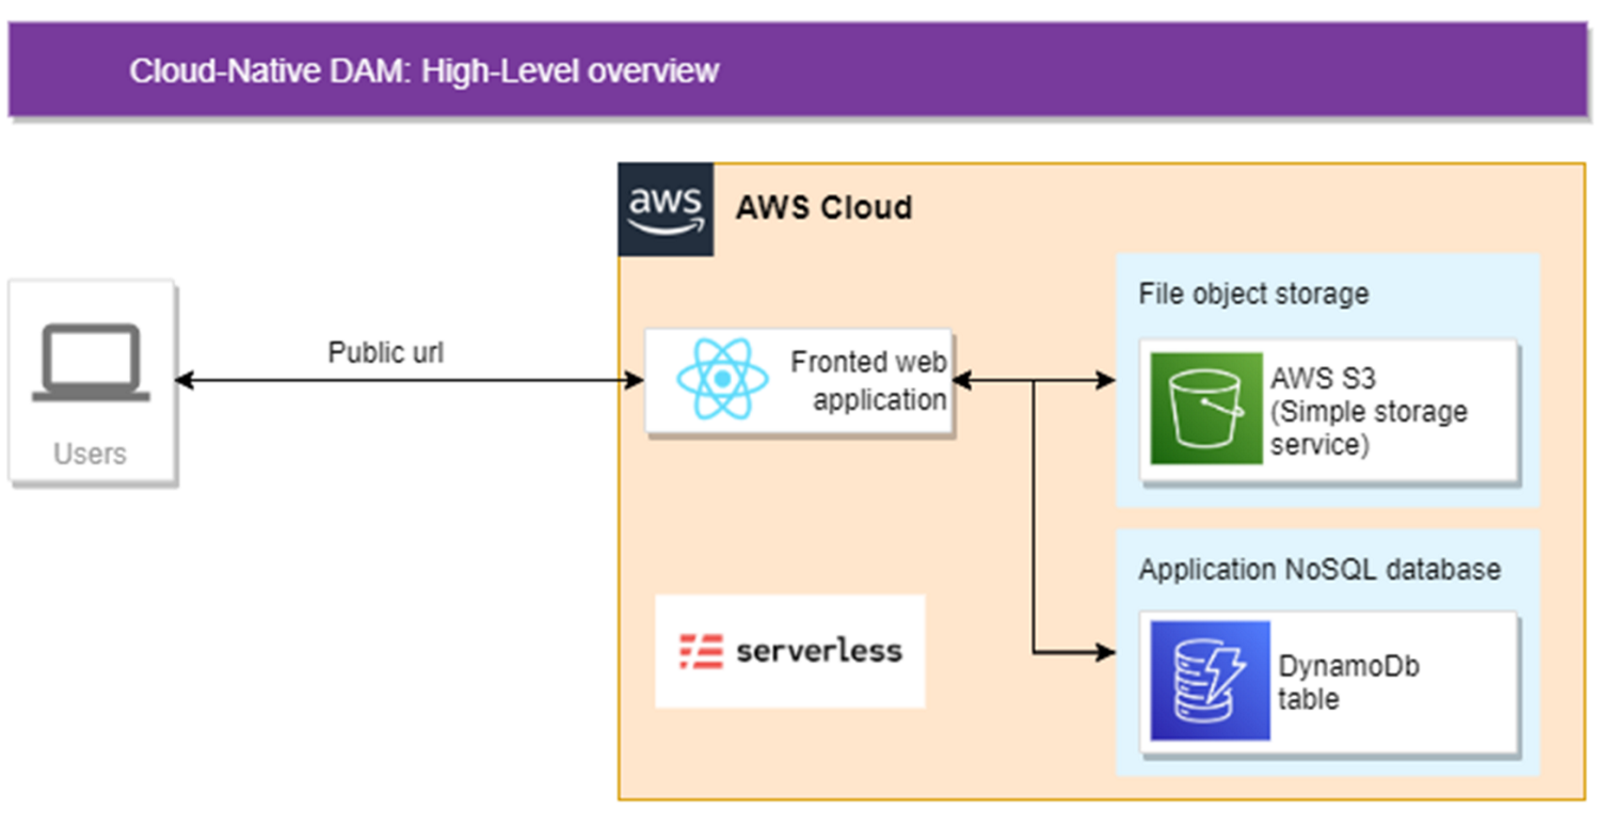
\includegraphics[scale=0.32]{images/HighLevelOverview.png}
    \caption{-- Общее описание архитектуры DAM"=системы}
    \label{highLevelOverview}
\end{figure}

Для создания этого Веб-приложения использовался фреймворк React, весь код написан на языке Typescript, который обеспечивает строгую типизацию и позволяет создавать структуры для облегчения поддержки и дальнейшей модернизации всего фронтенда. Для загрузки файлов в DAM-систему в приложении предусмотрено облачное хранилище для любых типов объектов. Для работы с метаданными, правами пользователей и остальными элементами DAM"=системы данное приложение использует NoSQL базу данных, разработанную компанией Amazon – DynamoDB. Использование правильного моделирования данных позволяет хранить разные структуры в одной таблице. Более детально и подробно устройство схемы базы данных будет рассмотрено в структуре бекэнда.

Архитектура этого веб-приложения не имеет ни одного сервера, нет облачных компьютеров, к которым была бы необходимость подключаться и управлять какими-либо аспектами приложения. Все используемые сервисы управляются и поддерживаются AWS, что позволяет при разработке уделять время только созданию ключевых частей программы, таких как: фронтенд, написанный на Typescript, Lambda функции на Python, принимающие REST-запросы через API Gateway и работающие с DynamoDB, AWS SDK для NodeJS, позволяющий управлять файлами в облаке, находящимися в S3 (simple storage service), что тоже является Serverless сервисом.

\subsection{Этапы разработки и компоненты приложения} 

Перечислим компоненты разработанной DAM"=системы, которые являлись различными стадиями в процессе реализации решения задачи, поставленной в ВКР.

Пользовательский интерфейс для управления и доступа к Digital Asset Management системе. Веб-приложение, созданное при помощи фреймворка React. AWS-сервис Amplify для непосредственного размещения сайта (на данный момент с тестовым бесплатным доменом, который выдаёт Amazon cloud провайдер).

Хранилище загружаемых в DAM"=систему файлов - AWS S3 service, позволяющий хранить файлы любого размера и предоставляющий API для их загрузки и скачивания. Использование AWS JavaScript SDK для работы с S3 сервисом на стороне пользовательского интерфейса.

Не реляционная база данных AWS DynamoDB для быстрого управления метаданными файлов, информации о smart-папках, структурирования файлов и правами пользователей. Разработка API приложения, создание запросов при работе пользователя с DAM"=системой через интерфейс. Обработка запросов на стороне облака с помощью AWS API Gateway. Разработка AWS Lambda-функций на языке Python для работы с базой данных - обращения, возвращения запрашиваемой информации и внесения изменений.

Программный код для автоматизации запуска DAM"=системы. Реализация подхода Infrastructure as code, создание AWS CloudFormation template, где описывается вся инфраструктура, необходимая для работы системы управления цифровыми активами. Написание Shell script и Python script для автоматизации запуска процесса сборки и развертывания приложения в облаке AWS.

\noindent 

\subsection{Пользовательский интерфейс}

Рассмотрим более подробно как устроен фронтенд разработанного приложения. Благодаря тому, что тип веб-сайта в данном случае Single Page Application, в один момент времени загружаются лишь только необходимые элементы страницы, которые запрашивает пользователь из-за чего ускоряется обработка запросов, и отображение самого контента на странице браузера.

Весь код был выполнен на языке TypeScript что позволяет легко понимать как работает тот или иной компонент приложения и что ему нужно. Рассмотрим все части более подробно.

После перехода по основной ссылке (без параметров), пользователь попадает на первую страницу: Home.tsx. Здесь находится лишь текст приветственного сообщения и кнопка перехода на страницу авторизации (которая предоставляется сервисом AWS Amplify). Также стоит заметить, что благодаря использованию библиотек для React отображения всех компонентов, всегда есть возможность полностью поменять оформление сайта без каких-либо крупных изменений в коде, это значительно ускоряет процесс разработки приложения.
В компоненте App.tsx расположена вся конфигурация приложения - роутеры различных путей ссылок и верхняя панель управления приложением: кнопки перехода на главную страницу, на страницу личного профиля и на элемент просмотра всех загруженных в облако файлов.

Все остальные страницы веб-сайта могут быть доступны только авторизированным пользователям, поэтому путь к ним будет состоять из <URL>/private/<Название страницы>

Первой страницей, которую увидит пользователь, будет PersonalPage.tsx (рисунок \ref{personalPage}).
\begin{figure}[H]
    \centering
    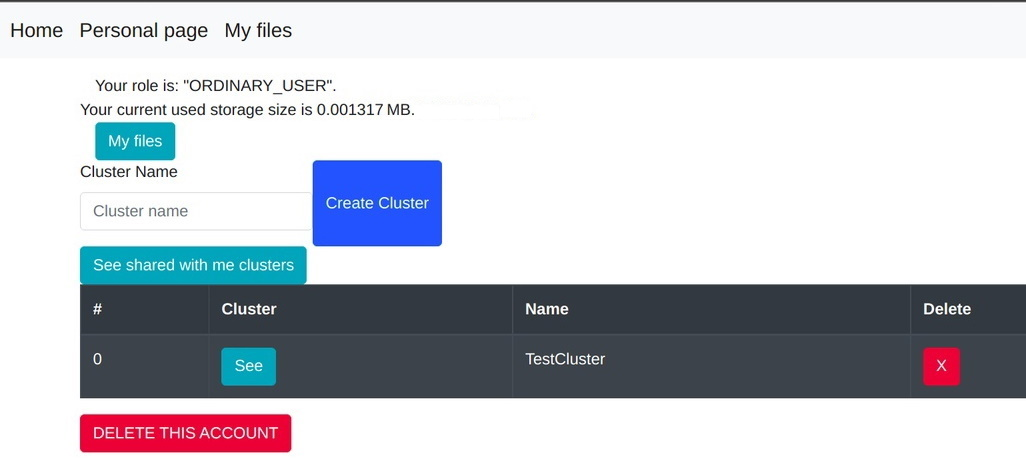
\includegraphics[scale=0.63]{images/ui/1_PersonalPage.jpg}
    \caption{-- Персональная страница пользователя}
    \label{personalPage}
\end{figure}

На ней находятся: панель управления личным профилем, поле для создания нового кластера, кнопка для перехода на страницу просмотра доступных пользователю smart-папок, таблица созданных кластеров и кнопка удаления всего пользовательского профиля. Также на этой странице указывается какое количество мегабайт использовано для хранения загруженных файлов.
Если же роль пользователя имеет привилегии администратора, то дополнительно будет отображаться компонент для отправки запроса напрямую в базу данных.
При подключении этой страницы происходит установка JWT токена авторизации (об этом будет рассказано далее), производится запрос в базу данных для получения всех smart-папок пользователя, а также запрос на получение информации о размере использованного хранилища.

При нажатии на отображаемый в списке кластер, произойдет переход на страницу просмотра соответствующей smart-папки: ClusterOverview.tsx (рисунок \ref{clusterPage}).
\begin{figure}[H]
    \centering
    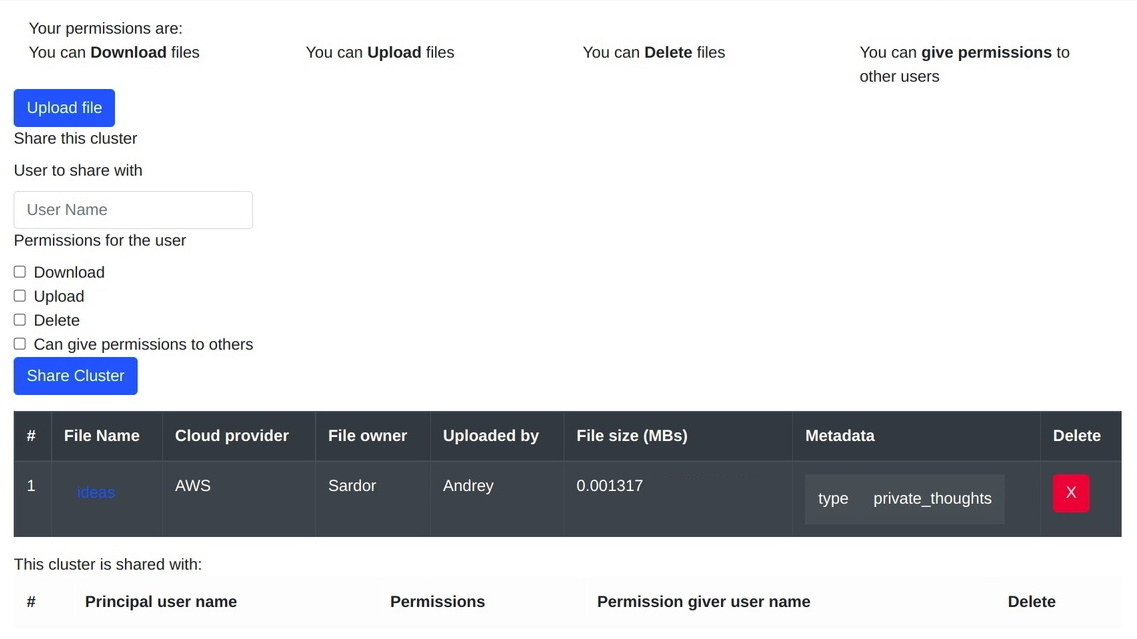
\includegraphics[scale=0.6]{images/ui/2_ClusterPage.jpg}
    \caption{-- Страница просмотра кластера}
    \label{clusterPage}
\end{figure}

Идентификатор smart-папки извлекается из url параметров, затем загружается токен авторизации, происходит запрос в базу данных для получения прав этого пользователя на указанный кластер, метаданных всех файлов добавленных в этот кластер и пользователей, которым также доступен этот кластер.

Для поиска и просмотра всех загруженных файлов существует страница SearchFiles.tsx как показано на рисунке \ref{filesPage}.
\begin{figure}[H]
    \centering
    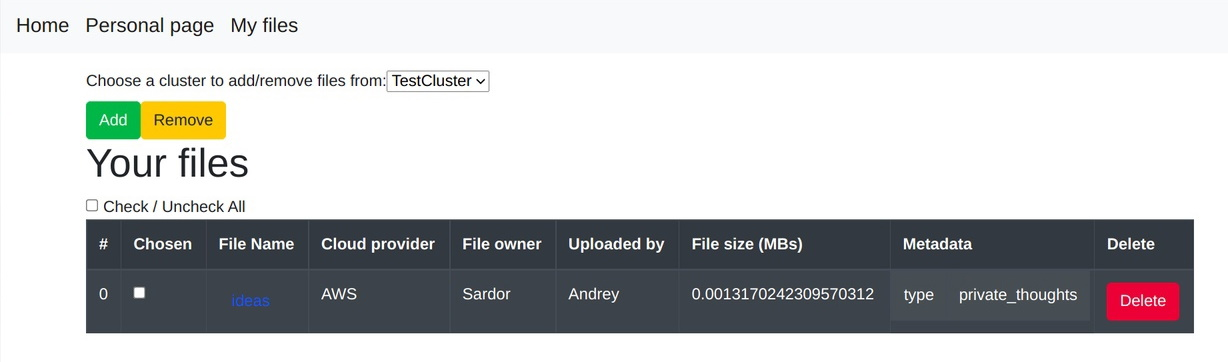
\includegraphics[scale=0.53]{images/ui/3_FilesPage.jpg}
    \caption{-- Страница просмотра загруженных пользователем файлов}
    \label{filesPage}
\end{figure} 

Здесь происходит получение всех файлов текущего пользователя, его кластеров и smart-папок, к которым есть доступ. Функционал данной страницы позволяет управлять размещением файлов по всем кластерам, осуществить поиск по характеристикам и удалять файлы из облака.
Благодаря использованию React был создан компонент FileOverview.tsx, который включает в себя всё представление отображения информации о файле. Это повышает инкапсуляцию кода, ускоряет разработку программы и позволяет разделить логику для лучшего понимания.
Также все основные функции запросов и обработки ответа от базы данных были вынесены в отдельный интерфейс componentsFunctons.ts, например: получение всех кластеров пользователя, метаданных файлов и функция скачивания файла из облака, использующая AWS SDK для JavaScript. Все типы данных, находящиеся в DynamoDB описаны как интерфейсы в databaseTables.ts, что позволяет видеть все поля объектов и открывает новые возможности при работе с типизированным кодом. Всё это было достигнуто благодаря использованию языка программирования TypeScript.

Наиболее удачной реализацией достоинств этого языка является написанная полиморфная функция для создания http запросов и обработки ответа, используя указанный тип объекта. Асинхронная функция makeFetch<T>
(fetchParams: FetchParams): Promise<T> принимает в качестве параметра объект типа FetchParams, где указывается url, метод запроса, токен авторизации и тело запроса (если таковое имеется). Возвращаемый результат зависит от указанного типа T, что позволяет эффективно интегрировать эту функцию в код приложения.

\subsection{Архитектура фронтенда, аунтефикации и REST API}
На рисунке \ref{authentication} изображена структура аунтефикации запросов с клиентской части приложения.
\begin{figure}[H]
    \centering
    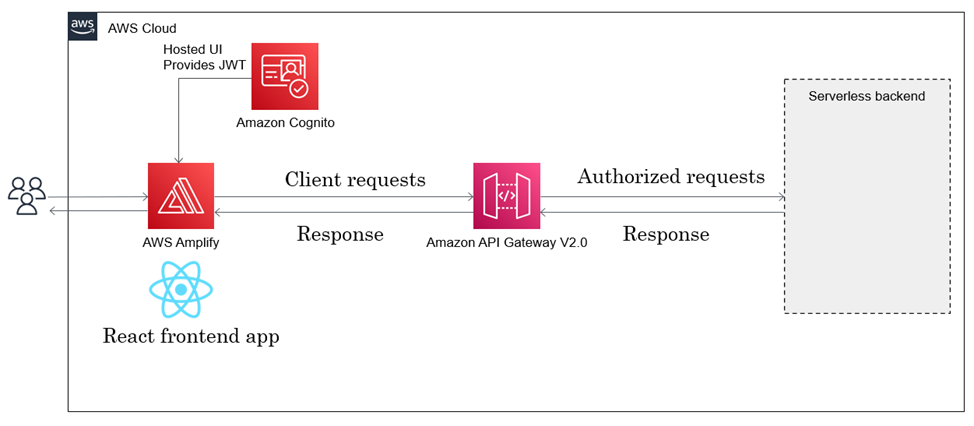
\includegraphics[scale=0.65]{images/Authentication.png}
    \caption{ -- Архитектура аунтефикации пользовательских запросов}
    \label{authentication}
\end{figure}

Для аунтефикации пользователей данное приложение использует JWT токены, которые предоставляет AWS сервис Cognito. Также этот сервис даёт возможность быстрого создания и настройки интерфейса для регистрации новых пользователей с проверкой почты. Во время создания всей системы в конфигурации указываются параметры создания Cognito UserPool, где будут храниться все данные о зарегистрированных пользователях, а также создается UserPoolClient для предоставления JWT токенов, здесь же указываются все ссылки на веб-приложение, развернутое в Amplify. Стоит заметить, что доступ в данном случае происходит по протоколу https, это позволяет защитить информацию при авторизации пользователей.

AWS Amplify – это сервис, предоставляющий недорогой хостинг веб-сайтов, за кадром используются еще несколько Amazon сервисов, но необходимо лишь настроить все свойства и указать как именно нужно развернуть фронтенд из директории с кодом всего приложения. Также есть возможность указать своё доменное имя.

AWS API Gateway позволяет использовать REST API вместе с Lambda функциями для общения веб-части приложения с базой данных. Вторая версия API Gateway даёт возможность прямо во время получения запроса проверить JWT токен и его подлинность автоматически, это встроенная возможность и требует лишь правильной настройки при запуске. Во время создания API Gateway, в конфигурации указывается провайдер токенов - в данном приложении это AWS Cognito, что позволяет эффективно использовать интеграцию этих двух сервисов облака AWS. 

Все описанные сервисы кроме Amplify создаются и подключаются друг к другу при помощи AWS CloudFormation, так как фронтенд настраивается немного иначе и сначала должен быть скомпилирован в Javascript и собран. CloudFormation позволяет создавать и поддерживать архитектуру в облаке Amazon в виде кода, а также разворачивать все ресурсы одним кликом мыши. Конфигурация каждого сервиса по отдельности тоже указывается в виде кода в CloudFormation template.

Далее перечислены основные npm (node packet manager) команды, доступные в корневой папке проекта:
\begin{enumerate}
\item build --- удаляет собранный проект в папке build/ (если таковая имеется) и запускает процесс сборки проекта с использованием webpack, что позволяет эффективно управлять этим процессом;
\item deploy --- запускает Shell script, который отвечает за полный процесс запуска DAM"=системы в облаке (процесс разворачивания приложения будет подробно рассмотрен в соответствующей главе);
\item start-webpack: запускает сборку проекта и сервер в development конфигурации, в данном случае связи с облачным провайдером не будет, используется для тестирования компонентов пользовательского интерфейса.
\end{enumerate}

\subsection{Хранение JWT токенов}

При работе данного программного продукта существенным фактором является правильное управление состоянием React приложения. Для этой цели используется Redux библиотека, позволяющая централизованно управлять общим хранилищем веб-приложения, где содержится такая информация, как: токен авторизации, токен идентификации и переменная, отвечающая за состояние загрузки страниц. В работе благодаря использованию Redux было эффективным образом реализовано получение доступа к этим данным из любой части SPA, написанного на React, а также их обновление. Вся работа с JWT токенами сопровождается обращением к reducer, который обеспечивает отслеживаемое и определенное изменение общего состояния приложения, связанного с авторизацией пользователя.

В файле reducer.ts находиться вся логика обработки событий, связанных с получением и сохранением JWT токенов.

\subsection{API Gateway}

Весь процесс общения пользовательского интерфейса с базой данных происходит через API приложения, точкой доступа к которому является AWS API Gateway. Этот сервис предоставляет endpoint для отправления запросов с клиентской части. Стоит заметить, что в конфигурации при разворачивании DAM"=системы указывается разрешенный источник этих запросов, где устанавливается тот домен, который предоставляет AWS Amplify и где соответственно находится весь фронтенд. Это позволяет существенно улучшить защиту приложения от атак, так как запросы может отправлять только запущенное по данному адресу React веб-приложение.
\clearpage

% Рассмотрим все доступные API запросы:
% \begin{enumerate}
%     \item /admin 
%     \begin{enumerate}
%         \item POST
%     \end{enumerate}
%     \item /clusters 
%     \begin{enumerate}
%         \item POST
%         \item GET
%         \item /\{proxy*\} 
%         \begin{enumerate}
%             \item GET
%         \end{enumerate}
%         \item DELETE 
%     \end{enumerate}
%     \item /files
%     \begin{enumerate}
%         \item POST
%         \item GET
%         \item /\{proxy*\} 
%         \begin{enumerate}
%             \item GET
%         \end{enumerate}
%         \item DELETE 
%     \end{enumerate}
%     \item /permissions 
%     \begin{enumerate}
%         \item POST
%         \item GET
%         \item /\{proxy*\} 
%         \begin{enumerate}
%             \item GET
%         \end{enumerate}
%         \item DELETE 
%     \end{enumerate}
%     \item /users
%     \begin{enumerate}
%         \item POST
%         \item DELETE 
%     \end{enumerate}
% \end{enumerate}

\subsection{Архитектура бекэнда}
На рисунке \ref{backend} изображены все функции обработки пользовательских запросов. Так как данное приложение разрабатывалось по методологии Serverless, все элементы не нуждаются в серверах: AWS Lambda функции запускаются при помощи AWS API Gateway только лишь при поступлении событий со стороны пользовательского интерфейса, далее эти функции обращаются к базе данных (которая также является Serverless сервисом) и выполняют необходимые действия. Вся деятельность при работе приложения распределена на указанное количество Lambda.
\begin{figure}[H]
    \centering
    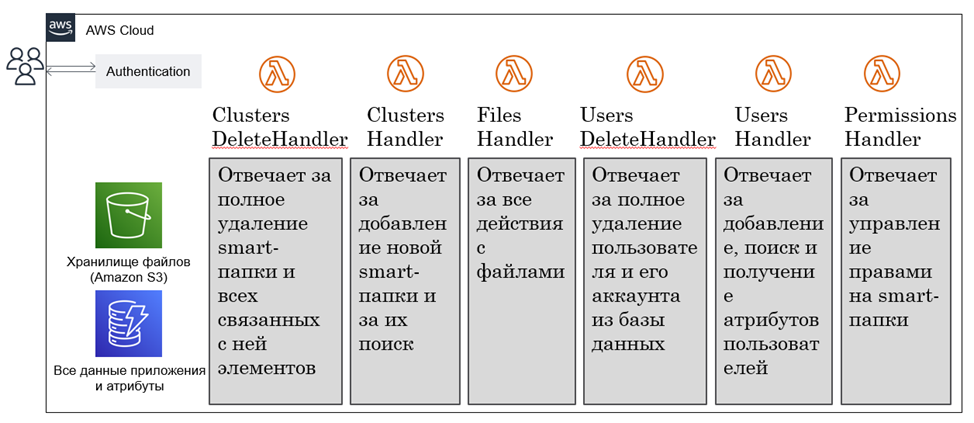
\includegraphics[scale=0.65]{images/BackEnd.png}
    \caption{-- Схема обработчиков запросов и работы с данными в DAM"=системе}
    \label{backend}
\end{figure}

В S3 хранилище находятся загруженные в DAM-систему файлы, с именами в виде индексов, которые назначает данное приложение при добавлении нового файла в базу данных. При загрузке нового файла на странице UploadFile.tsx происходит обработка метаданных, указанных пользователем, проверяется количество уже занятого места в облаке (если добавление файла приведет к превышению указанного в конфигурации DAM"=системы лимита, загрузка файла завершиться с ошибкой и предложением докупить место в облачном хранилище). Затем, используя AWS JavaScript SDK, происходит загрузка в соответствующее S3 хранилище, созданное при разворачивании системы управления цифровыми активами.

Для работы с DynamoDB используется сервис AWS Lambda, который имеет возможность подключения к AWS API Gateway и каждая из Lambda функций является обработчиком одного или нескольких REST запросов с клиентской части приложения. Распределение нагрузки выполнения этих запросов было удачно реализовано так, чтобы избежать слишком долгой обработки задачи одной функцией, что может вызвать увеличение стоимости, а также чтобы не было огромного количества кода в одном файле, что усложняет поддержку и добавление нового функционала.

Рассмотрим каждую Lambda-функцию и её задачи.

Обработчик запросов работы с информацией о пользователях DAM"=системы: UsersHandler.py. Извлекает из запроса идентификатор пользователя (обработка JWT токена и его расшифровка происходит на стороне AWS API Gateway). Совершает запрос в базу данных на поиск соответствующего пользователя. Удачная реализация состоит в том, что нет необходимости прикреплять обработчик на сервис AWS Cognito при создании нового пользователя. Так как Lambda функция может быть запущена только через API Gateway, который предварительно проверяет JWT токен на подлинность, то при отсутствии записи о пользователе в базе данных, текущий обработчик сразу может сделать вывод, что необходимо добавить новую запись в базу данных, так как JWT токен подтверждает что идентификатор является подлинным. Если же данный пользователь уже занесен в базу данных, то этот обработчик вернет в качестве ответа роль этого пользователя.

Обработчик запросов работы с кластерами пользователя: ClustersHandler.py. Извлекает из запроса идентификатор пользователя. Если это POST запрос и в теле запроса нет идентификатора кластера, это говорит о том, что необходимо создать новую smart-папку. Генерируется уникальный идентификатор нового кластера и в базу данных добавляется запись с указанием имени, идентификатора кластера и пользователя, который им владеет. Если это GET запрос и параметров запроса нет, то в базу данных отправляется запрос найти все smart-папки указанного пользователя. Если же параметры запроса указаны, то необходимо найти именно тот кластер, идентификатор которого установлен, а также данная функция определяет, является ли пользователь, запрашивающий данный кластер, его владельцем.

Обработчик запросов работы с метаданными файлов DAM"=системы: FilesHandler.py. Извлекает из запроса идентификатор пользователя, если это POST запрос и в теле запроса поле "action" пустое, это говорит о том, что необходимо добавить файл в указанный кластер. Генерируется уникальный идентификатор новой записи о метаданных файла и в базу данных формируется транзакция, добавляющая как сам файл, так и информацию о том, в какой кластер он был добавлен, по той причине, что нельзя добавить файл не указав к какой smart-папке он относится. Далее происходит обновление записи о метаданных файла - указываются все пользовательские теги. Удачная реализация состоит в том, что при возникновении ошибки хотя бы в одном из этих действий, оба будут отменены так как это транзакция и Lambda-функция вернет сообщение об ошибке. Если это POST запрос и в теле запроса поле action равно addFileToCluster, то в базу данных отправляется запрос на создание записи кластер"=файл, тем самым метаданные указанного файла привязываются к соответствующему кластеру. Все значения идентификаторов извлекаются из тела запроса. Если это GET запрос и параметров запроса нет, то необходимо найти все файлы, загруженные пользователем, идентификатор которого был получен в самом начале работы Lambda"=функции. При поступлении GET запроса с параметром calcUsedSize=true, происходит подсчет общего использованного места в облаке данным пользователем. Благодаря хранению размера файла появляется возможность быстро и эффективно произвести данную операцию. При поступлении GET запроса с параметром clusterId, рассматриваемая функция возвращает все метаданные файлов, которые привязаны к соответствующему кластеру. Сначала в базу данных отправляется запрос найти все записи кластер"=файл для указанного идентификатора smart-папки. Затем, проходя по каждому из элементов в ответе, в базу данных поступает новый запрос на поиск соответствующих метаданных файла. После этого вся информация отправляется на пользовательский интерфейс. При поступлении DELETE запроса из базы данных удаляется соответствующая информация о файле или связка кластер"=файл (при откреплении файла от smart-папки).

Аналогично работает функция управления правами на использование smart-папок PermissionsHandler.py. Функции удаления записей из базы данных (ClustersDeleteHandler, UsersDeleteHandler) работают по той же системе, как и удаление в FilesHandler.py.

Стоит также заметить, что код Lambda"=функций эффективно обрабатывает все возможные ошибки при работе с базой данных DynamoDB и передает ответ пользовательскому интерфейсу, который отображает детали возникшей ошибки.

\subsection{База данных DAM"=системы}
На рисунке \ref{dbSchema} изображена схема используемой базы данных - атрибуты, их названия, а также как именно они связаны между собой и с помощью каких полей происходит агрегация данных при различных запросах (global и local secodary indexes).
\begin{figure}[H]
    \centering
    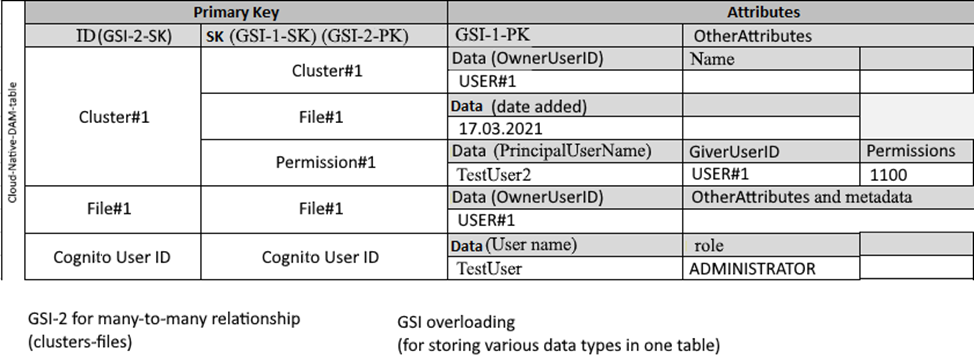
\includegraphics[scale=0.65]{images/DbSchema.png}
    \caption{-- Схема базы данных}
    \label{dbSchema}
\end{figure}

В вышеупомянутой схеме указывается как распределена вся информация по таблице во время работы приложения. Рассмотрим более подробно процесс агрегации данных.

Использование основных Primary Key и Sort Key таблицы DAM"=системы в DynamoDB. Рассмотрим запрос на получение кластера по указанному идентификатору.
\begin{lstlisting}
query_params = {
    'TableName': 'CloudNativeDAM_DB',
    'ExpressionAttributeNames': {'#ID': 'ID', '#SK': 'SK'},
    'ExpressionAttributeValues': {':id': {'S': cluster_id},':sk': {'S': cluster_id}},
    'KeyConditionExpression': '#ID = :id AND #SK = :sk'
}
\end{lstlisting}
TableName - имя таблицы, так как эффективность DynamoDB позволяет использовать для всех операций DAM"=системы одну таблицу, значение этого параметра будет всегда равно названию системы управления цифровыми активами.

ExpressionAttributeNames - переименование названий атрибутов во избежание конфликтов строковых обозначений. Здесь происходит обращение к Primary Key "ID" и к Sort Key "SK".

ExpressionAttributeValues - значения атрибутов, по которым производиться поиск. В данном случае для ":id" и для ":sk" устанавливается строковое значение (о чем символизирует символ 'S') идентификатора кластера.

KeyConditionExpression - выражение поиска, в котором указываются ExpressionAttributeNames и ExpressionAttributeValues. Здесь атрибуты "ID" и "SK" должны быть одновременно равны ":id" и ":sk" соответственно.

Как видно из схемы базы данных Primary Key "ID" и Sort Key "SK" нужны для хранения различных типов данных в одной таблице - если "ID" и "SK" начинаются с \quotes{Cluster\#} , то в данной строке будет храниться вся информация о кластере (владелец, имя и тд). Если же "ID" начинается с \quotes{Cluster\#}, но "SK" начинается с \quotes{File\#}, то здесь подчеркивается добавление определенного файла в заданную smart-папку. Аналогично для "SK" начинающегося с \quotes{Permission\#} - права, закрепленные за конкретным кластером.

Использование GSI-1 (Data-index) для случая, когда появляется необходимость использовать другое поле в качестве Primary Key для агрегации необходимых данных (получить все кластеры для указанного пользователя). Так как Primary Key "ID" и Sort Key "SK" таблицы отвечают за тип записи в базе данных, то обращение к атрибуту, в котором содержится информация о владельце кластера не может быть выполнена, используя эту пару ключей. По этой причине был создан Global Secondary Index с Primary Key "Data" и с Sort Key "SK". Как можно заметить по схеме базы данных - в поле "Data" хранятся совершенно различные данные.

\clearpage

Рассмотрим запрос на получение всех кластеров для указанного пользователя.
\begin{lstlisting}
query_params = {
    'TableName': 'CloudNativeDAM_DB',
    'IndexName': 'Data-index',
    'ExpressionAttributeNames': {'#C_ID': 'SK', '#OWN': 'Data'},
    'ExpressionAttributeValues': {':Cid': {'S': 'CLUSTER#'},':Uid': {'S': requester_cognito_user_id}},
    'KeyConditionExpression': '#OWN = :Uid AND begins_with(#C_ID, :Cid)'
}
\end{lstlisting}

В данном случае ExpressionAttributeNames указывают на использование поля "Data". В ExpressionAttributeValues устанавливается критерий поиска, \quotes{:Cid='CLUSTER\#'}, так как значение поля "SK" должно начинаться с \quotes{CLUSTER\#}, таким образом можно однозначно сказать, что эта строка несет в себе информацию о кластере. KeyConditionExpression находит все записи в базе данных, где "Data" равна идентификатору владельца кластера, а поле "SK" начинается с \quotes{CLUSTER\#}.

Таким образом, по основному ключу, в котором хранится информация различных типов, есть способ отфильтровать данные по атрибуту "SK". В терминах AWS DynamoDB этот эффективный подход называется GSI overloading, что позволяет в одной таблице хранить данные, которые в традиционных реляционных базах данных приходилось хранить в разных.

Использование GSI-2 (File-Clusters-index). В базах данных существует еще одно отношение: многие ко многим, что в данной программе позволяет получить все кластеры, в которых находиться определенный файл, таким образом, обеспечивая обратную зависимость файл"=кластер. Для решения этой проблемы создается второй Global Secondary Index - \quotes{File-Clusters-index}, у которого ключи являются обратной парой основной таблицы: Primary Key - это "SK"\ , а Sort Key - это "ID".

\clearpage

Рассмотрим запрос на получение всех кластеров в которые был помещен указанный файл.
\begin{lstlisting}
query_params = {
    'TableName': 'CloudNativeDAM_DB',
    'IndexName': 'File-Clusters-index',
    'ExpressionAttributeNames': {'#C_ID': 'ID', '#F_ID': 'SK'},
    'ExpressionAttributeValues': {':Cid': {'S': 'CLUSTER#'},':Fid': {'S': file_id}},
    'KeyConditionExpression': '#F_ID = :Fid AND begins_with(#C_ID, :Cid)'
}
\end{lstlisting}

Как видно из кода, этот случай аналогичный первому, но выражения, связанные с файлами, поменялись местами с выражениями, связанными с кластерами.

Необходимость использования этого GSI обусловливается тем, что Primary Key всегда должен быть указан, по нему нет возможности запустить функцию "begins\_with", так как эта функция может быть использована только на Sort Key.

На рисунке \ref{gsis} изображены все индексы базы данных и информация о них.
\begin{figure}[H]
    \centering
    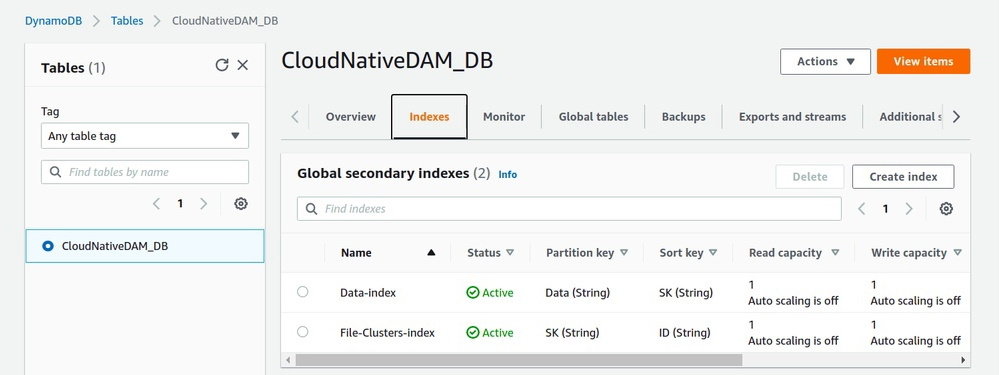
\includegraphics[scale=0.65]{images/gsis.jpg}
    \caption{-- Индексы в базе данных}
    \label{gsis}
\end{figure}

\subsection{Автоматизация разворачивания приложения}

Одним из основных преимуществ разработанного программного продукта является его автоматическое разворачивание в облачном провайдере. Для запуска достаточно начать выполнение одного Shell script, который включает в себя все аспекты инфраструктуры в AWS, а также подключения пользовательского интерфейса к ней.

Рассмотрим данный процесс более подробно. Для начала стоит заметить, что все облачные ресурсы находятся в так называемом template и выполнены с помощью языка Yaml. Сервис AWS CloudFormation использует этот template для создания всех указанных и сконфигурированных ресурсов в выбранном аккаунте Amazon Web Services. 

Далее перечислены компоненты файла InitialCloudFormationTemplate.yml:
\begin{enumerate}
\item ключи доступа к S3 хранилищу, в котором находятся все загруженные в DAM"=систему файлы;
\item полное описание API Gateweay, все методы и точки доступа, какие Lambda"=функции закреплены за каждым из REST запросов, права использования в AWS аккаунте для каждой из функций, а также описание интеграции предоставления JWT токенов из AWS Cognito;
\item путь к коду каждой из Lambda"=функций, так как это Serverless приложение, сам код будет архивирован и загружен в облако чуть позже;
\item все AWS IAM права для работы Lambda"=функций;
\item конфигурация сервиса Cognito для хостинга пользовательского интерфейса и интеграции с API Gateway, используя JWT токены;
\item настройка AWS Amplify;
\item значения на выход после создания ресурсов в облаке для дальнейшей настройки приложения и интеграции с AWS (идентификатор Amplify приложения, ключи доступа к S3, а также API Gateway endpoint и ссылка для регистрации).
\end{enumerate}


В корне репозитория с кодом данной DAM-системы содержится файл fullDeploy.sh, позволяющий запустить процесс, этапы которого перечислены ниже:
\begin{enumerate}
\item упаковка вышеупомянутого InitialCloudFormationTemplate.yml template"=файла и кода всех функций;
\item разворачивание упакованного template через AWS CloudFormation;
\item запуск generate\_config\_script.py для генерации конфигурационного файла для интеграции пользовательского интерфейса с облаком;
\item запуск generate\_amplify\_deployment\_script.py для генерации файла автоматического создания Amplify окружения, где указывается идентификатор созданного приложения;
\item далее происходит инициализация amplify в локальной папке с кодом проекта;
\item используя утилиту expect для Linux, в облаке создается хостинг инициализированного Amplify приложения;
\item последний шаг автоматизации - опубликовать пользовательский интерфейс, используя утилиту amplify.
\end{enumerate}

Как только последний шаг завершит своё выполнение, появляется возможность перейти по указанному адресу и попасть на основную страницу фронтенда приложения. Удачная реализация автоматизации разворачивания приложения предоставляет огромное количество значимых преимуществ - уменьшение ошибок при подключении DAM"=системы, огромное ускорение процесса дельнейшей разработки, упрощение процесса тестирования и так далее.

\subsection{Поиск среди загруженных файлов}
Данная система использует продвинутый сервис для поиска - OpenSearch, это модернизированная компанией Amazon версия программы с открытым исходным кодом, поддерживающая интеграцию с многими другими сервисами AWS. Была создана функция, индексирующая все добавленные файлы и их метаданные -- это позволяет осуществлять расширенный поиск. Например, по имени файла или по существованию тега, не обязательно по конкретному его значению. Все найденные элементы будут возвращены по релевантности. На рисунке \ref{searchExample} изображен пример поиска по метаданным.

\begin{figure}[H]
    \centering
    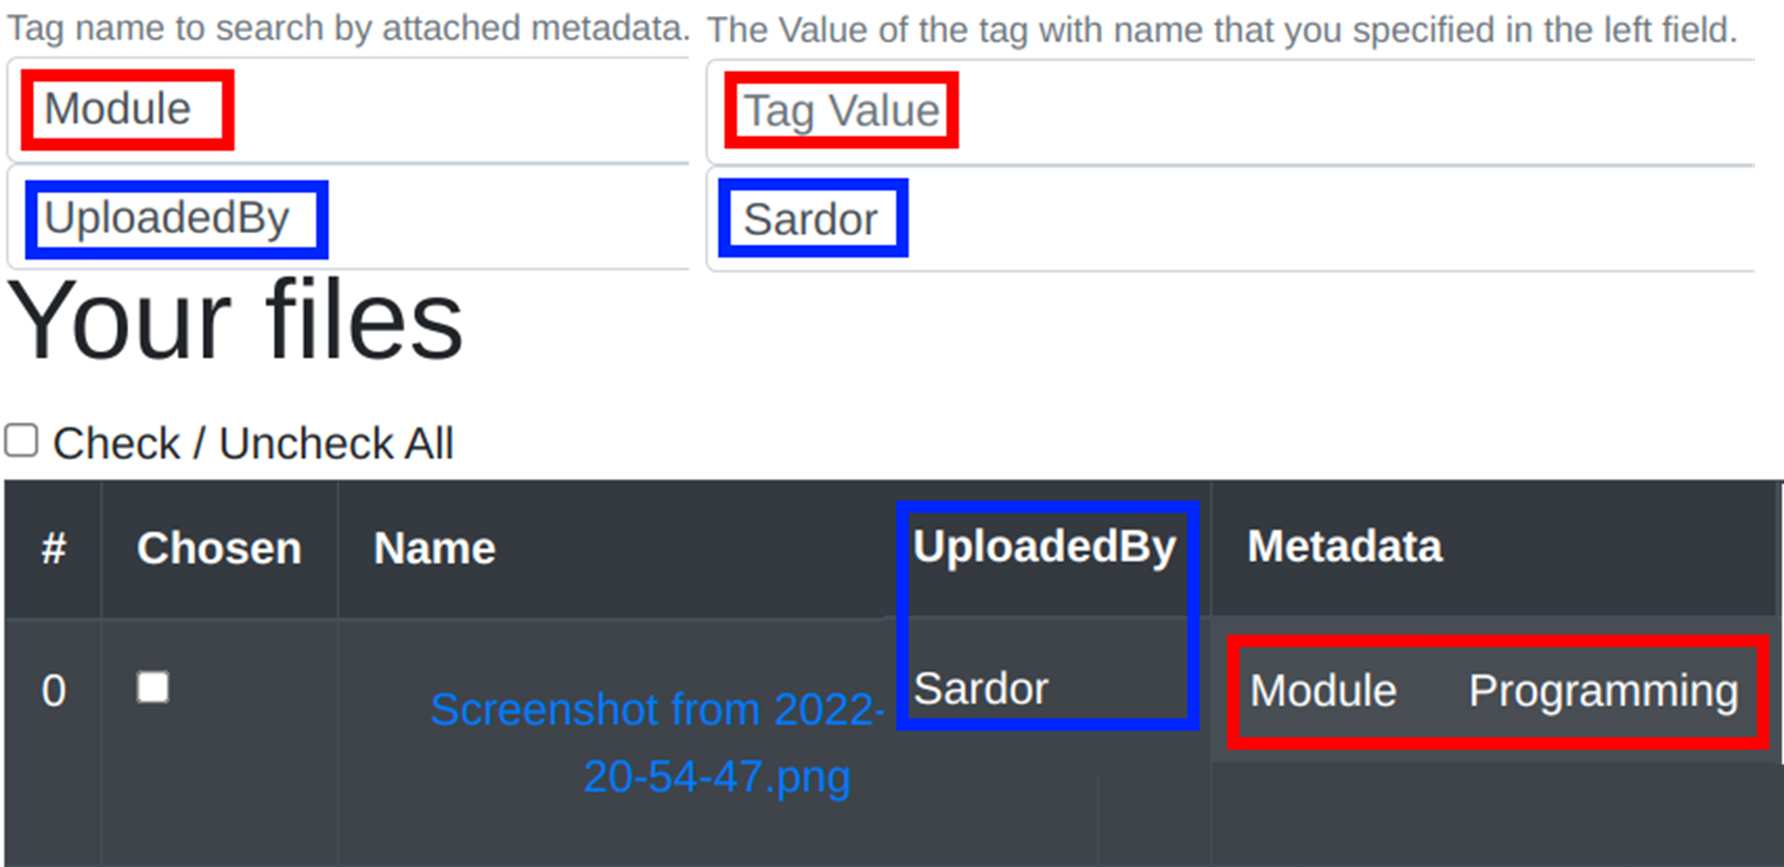
\includegraphics[scale=0.35]{images/ui/4_SearchExample.png}
    \caption{-- Поиск по метаданным}
    \label{searchExample}
\end{figure}

Полная архитектура приложения в облаке AWS, с учетом обработки поисковых запросов представлена на рисунке \ref{fullAwsArch}.

\begin{figure}[H]
    \centering
    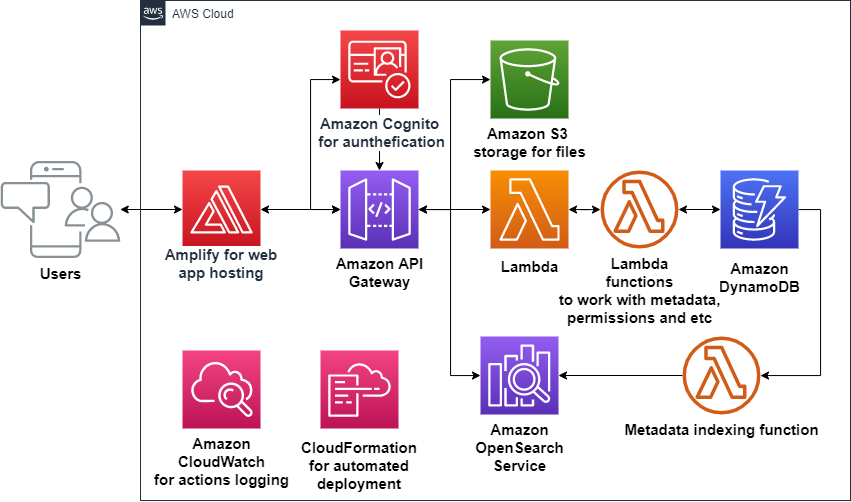
\includegraphics[scale=0.55]{images/fullArch.png}
    \caption{-- Полная архитектура DAM-системы в AWS}
    \label{fullAwsArch}
\end{figure}

\subsection{Пример работы приложения}

После успешной развертки DAM-системы, перейдя по ссылке на хостинг можно будет увидеть главную страницу, с которой, нажав на соответствующую кнопку, можно перейти на страницу авторизации, предоставляемой сервисом AWS Cognito. 

Далее перечислены доступные зарегистрированному пользователю действия:
\begin{enumerate}
\item посмотреть все загруженные файлы и распределить их по папкам;
\item создать новую smart-папку (рисунок \ref{personalPageMvp}) и увидеть все присутствующие кластеры;
\item перейти на страницу с отображением всех кластеров (smart-папок), которые этот пользователь может видеть, то есть те, на просмотр которых у данного пользователя есть права;
\item удалить полностью свой аккаунт со всеми файлами и smart-папками.
\end{enumerate}

\begin{figure}[H]
    \centering
    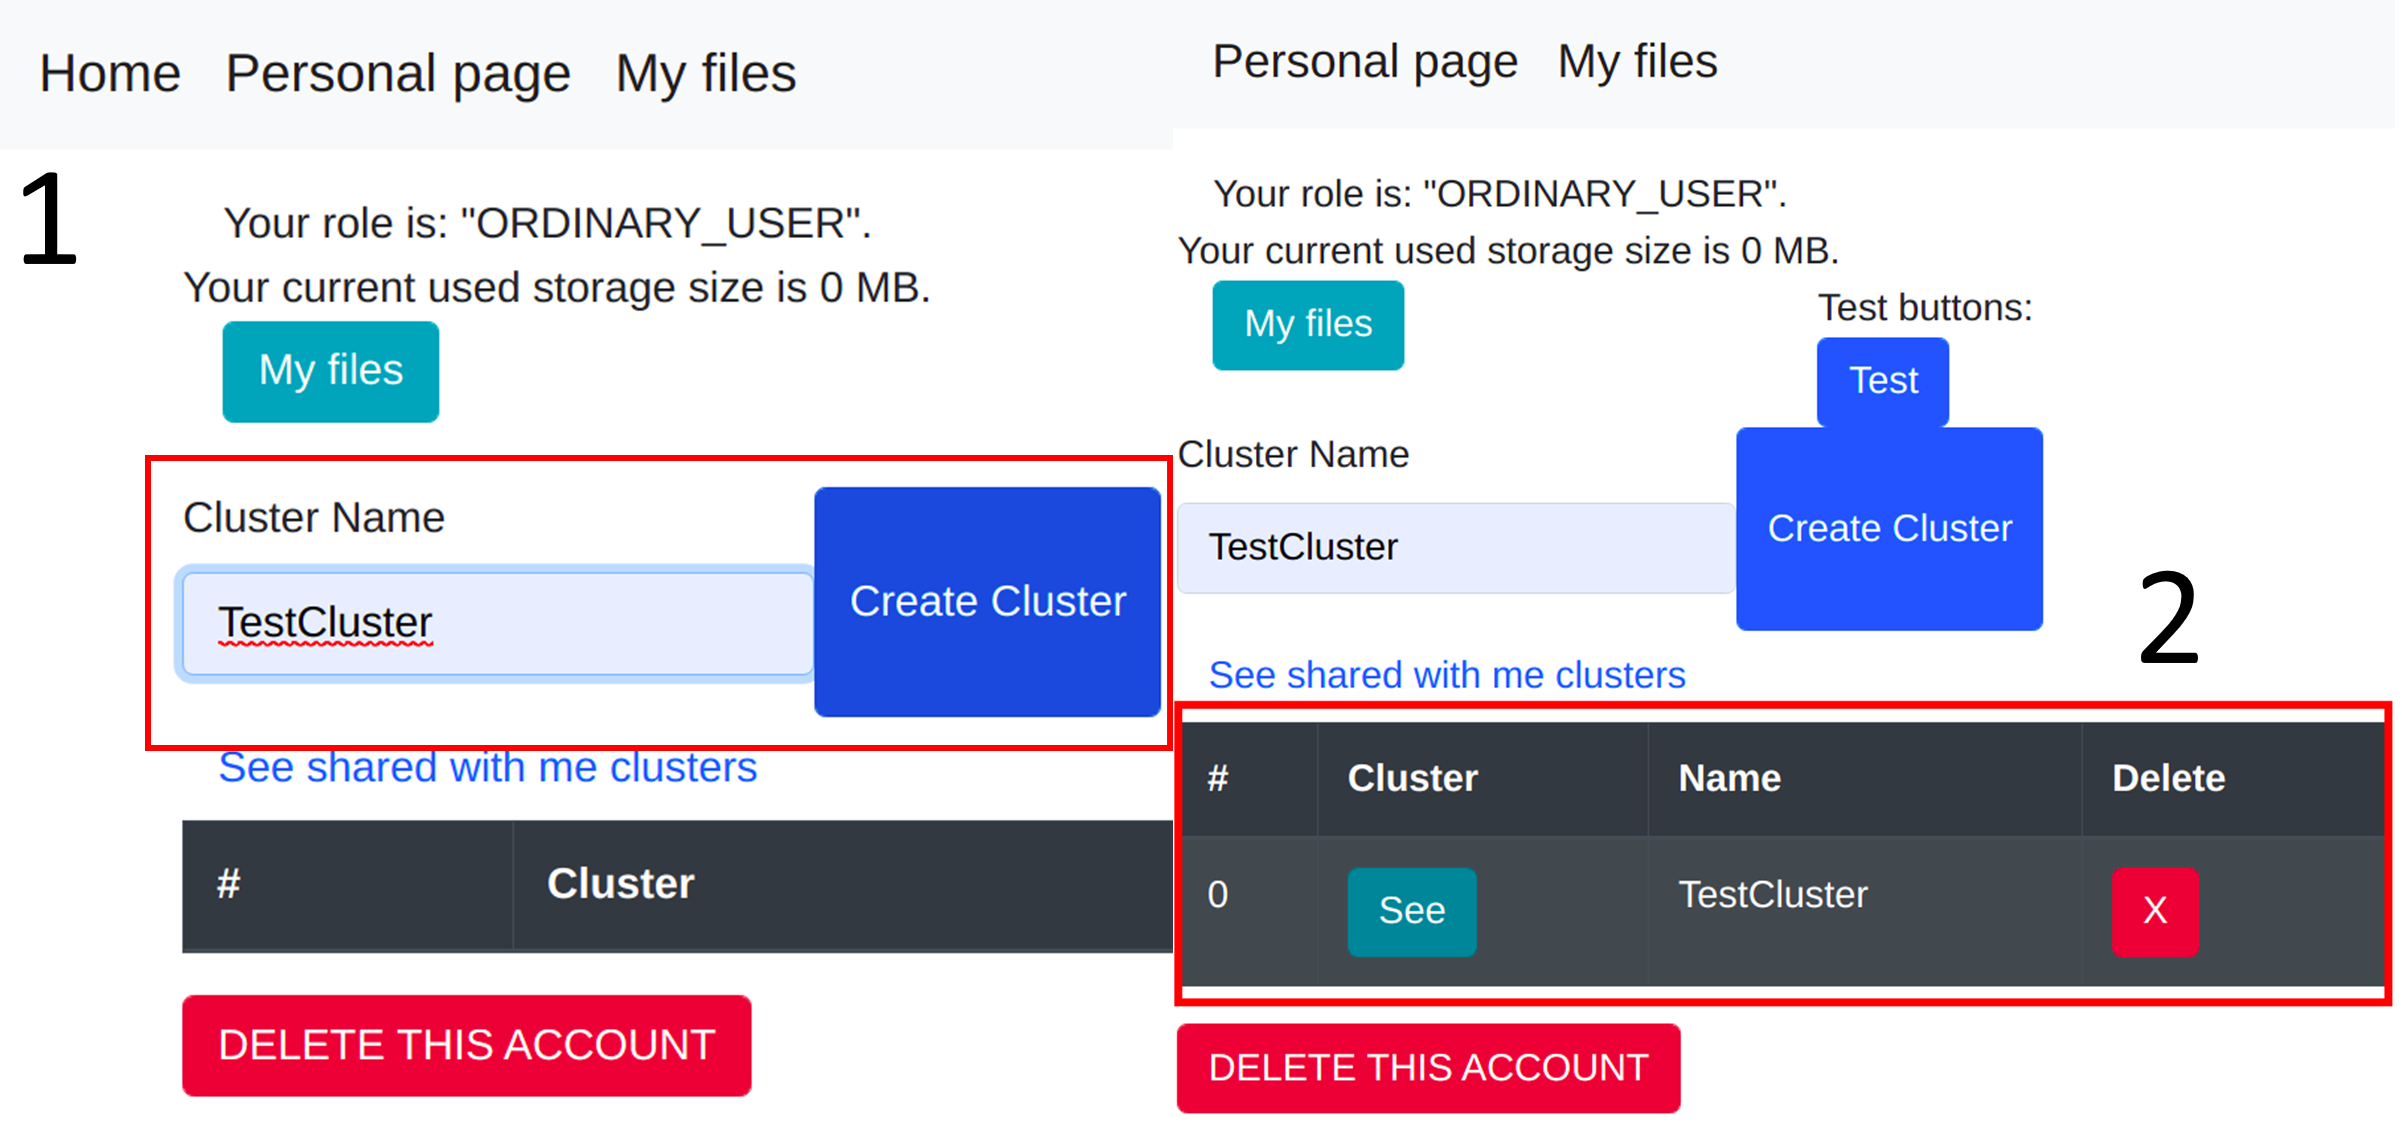
\includegraphics[scale=0.27]{images/mvp/1_CreateNewCluster.png}
    \caption{-- Создание нового кластера}
    \label{personalPageMvp}
\end{figure}

Перейдя на страницу просмотра кластера, пользователь увидит все доступные ему права – скачивание, загрузка в облако, удаление и выдача прав другим пользователям. Также будет возможность загрузить файл. При нажатии на кнопку \quotes{Upload File} откроется новая страница, где можно будет добавить любое количество метаданных к загружаемому файлу как показано на рисунке \ref{fileUpload}.

Также на странице просмотра кластера есть возможность выдать указанные права на доступ к этой smart-папке выбранному пользователю -- рисунок \ref{addPermissions}.

Другой пользователь, с которым поделились доступом к smart-папке может увидеть этот кластер, если нажмет на главной странице своего профиля на кнопку “See shared with me clusters”. Выбрав нужную папку, этот второй аккаунт будет иметь только те права, которые были указаны при добавлении доступа первым аккаунтом как показано на рисунке \ref{sharedCluster}.

\begin{figure}[H]
    \centering
    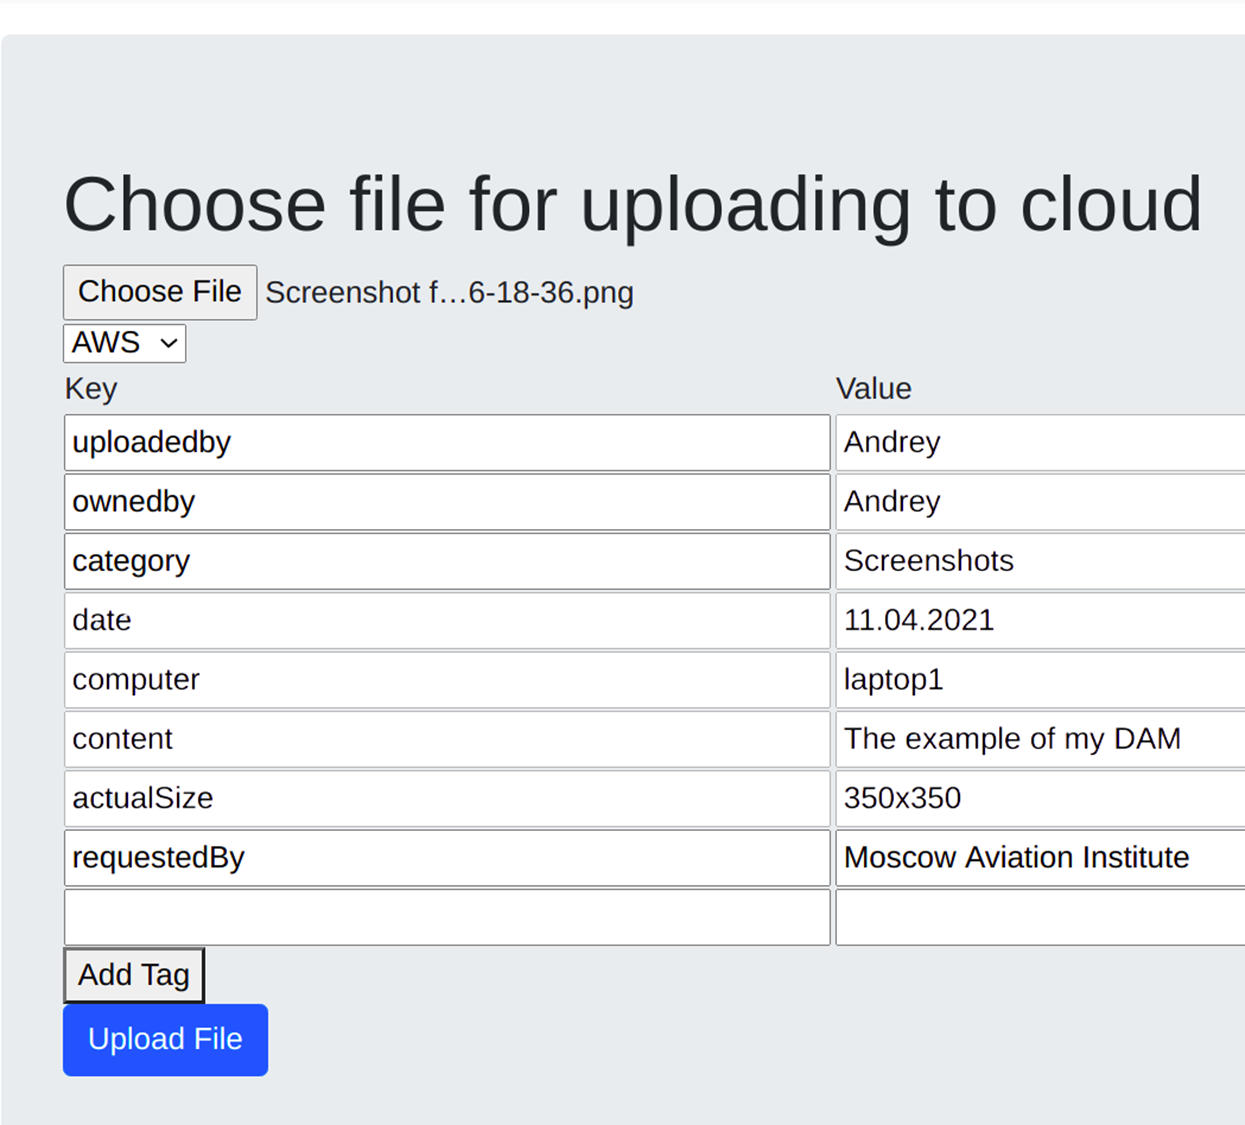
\includegraphics[scale=0.4]{images/mvp/2_ExampleFileUpload.png}
    \caption{-- Пример загрузки файла с указанием метаданных}
    \label{fileUpload}
\end{figure}

\begin{figure}[H]
    \centering
    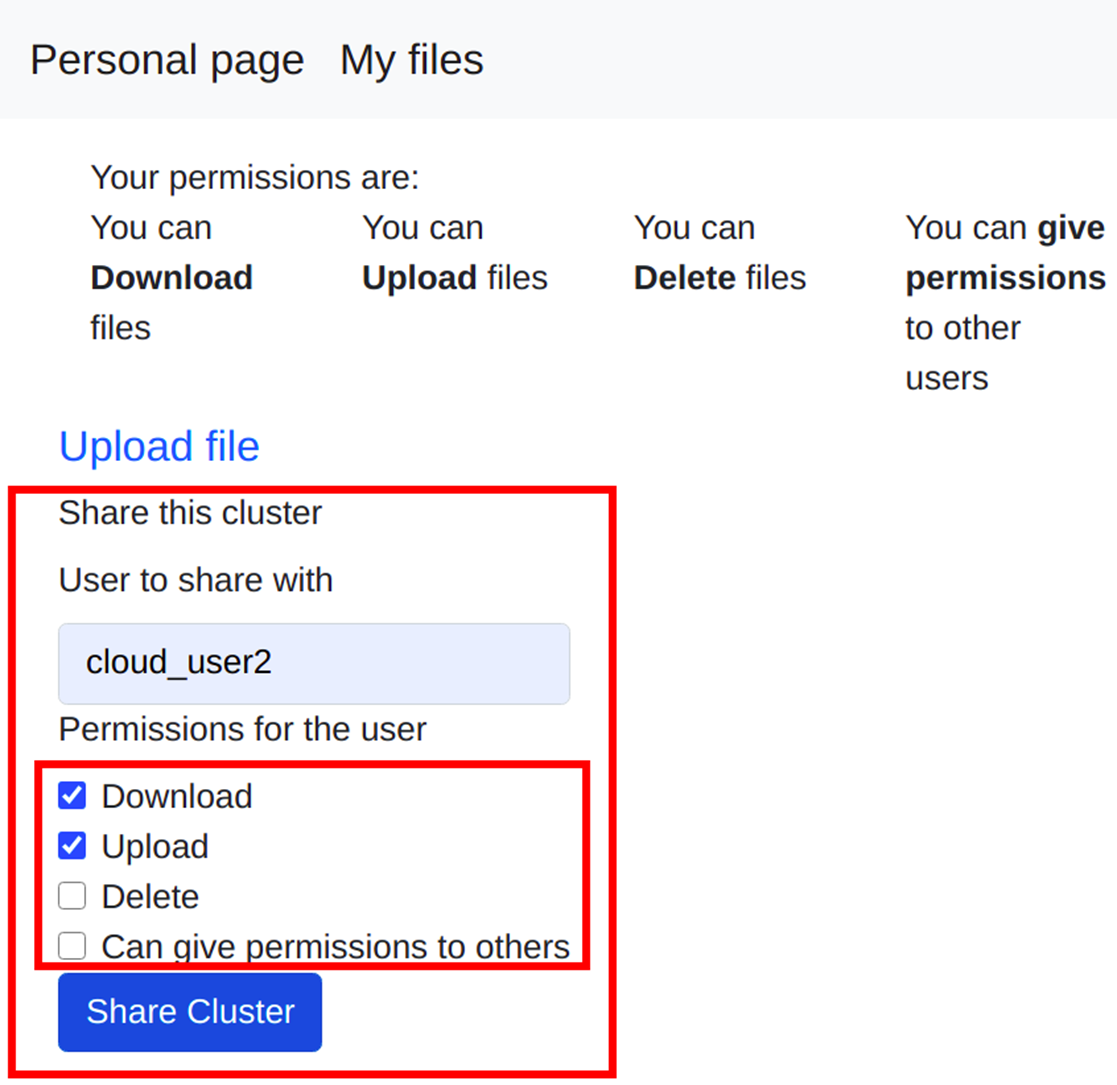
\includegraphics[scale=0.35]{images/mvp/3_GivePermissions.png}
    \caption{-- Выдача прав на владение кластером пользователю}
    \label{addPermissions}
\end{figure}

\begin{figure}[H]
    \centering
    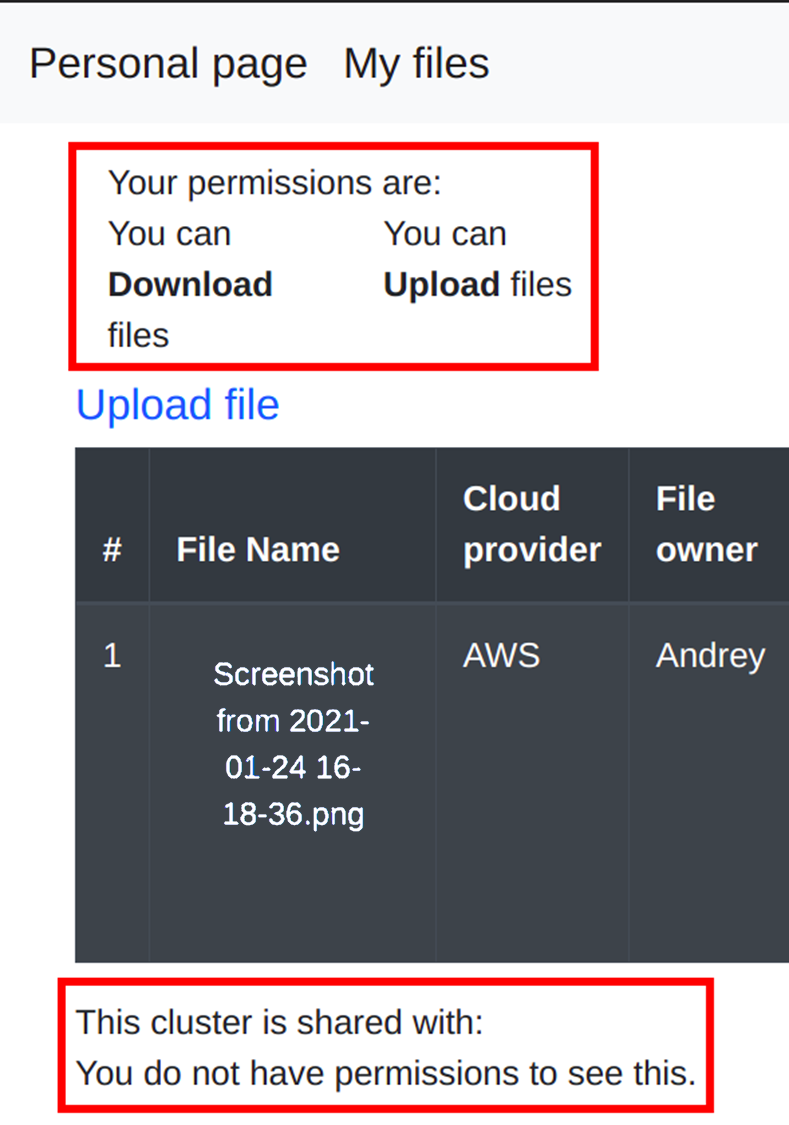
\includegraphics[scale=0.6]{images/mvp/4_SharedCluster.png}
    \caption{-- Просмотр кластера пользователем с ограниченными правами}
    \label{sharedCluster}
\end{figure}


\clearpage
% \chapter{ПРИМЕНЕНИЕ РАЗРАБОТАННОГО ПРОГРАММНОГО ПРОДУКТА}

\subsection{Опубликованный продукт}
На платформе GitHub опубликован весь код приложения в открытом доступе \cite{MySourceCode}. 

Также там присутствует описание запуска процесса развертывания DAM-Системы и краткие пояснения. Следуя указанной инструкции, в заданном AWS аккаунте будет создана описанная в данной работе система.

\prettypart{ЗАКЛЮЧЕНИЕ}
% \section{Положения, выносимые на защиту}
% \section{Результаты работы}


В работе были рассмотрены и исследованы различные подходы к созданию DAM"=систем. Практическим результатом работы является разработанная система управления цифровыми активами, реализованная с помощью новейших облачных технологий. 

Основным преимуществом этой DAM-системы является скорость разворачивания в AWS окружении и простота подключения, использования. Права пользователей хранятся в базе данных, а не в AWS IAM, что упрощает архитектуру в облаке и не дает информации о доступе к файлам выходить за пределы Digital Asset Management системы. 

Это реализованная cloud-native DAM-система, для работы которой необходим только аккаунт AWS, все расходы можно увидеть через свой AWS счёт. Оплата происходит только за реально используемые ресурсы и количество запросов, как при любом другом использовании Serverless архитектуры. Работа с метаданными обеспечивается с помощью такой базы данных как AWS DynamoDB и происходит через REST API, запросы к которому обрабатываются AWS Lambda функциями. Файлы оптимально размещены и структурированы с помощью кластеров (smart-папок), права на доступ к каждой папке могут быть выданы ровно в необходимом для работы количестве. Ограничений на загрузку и скачивание файлов нет, так как AWS управляет своими сервисами и масштабирует их по мере необходимости.
Благодаря AWS CloudFormation и логически разделенным AWS Lambda функциям есть возможность удобного способа поддержки и добавления нового функционала в данную DAM-систему.

Сформулированная задача была полностью решена в рамках выпускной квалификационной работы. Разработанный программный продукт возможно развивать и дальше, добавляя новый функционал и используя огромные возможности облака AWS, такие как мониторинг всех процессов системы, машинное обучение для добавления метаданных, различные улучшения производительности и доступности на региональном уровне, а также дополнительные возможности защиты приложения.

\newpage
% \medskip

%Sets the bibliography style to UNSRT and imports the 
%bibliography file "samples.bib".
% \bibliographystyle{unsrt}
% \bibliography{Lib}
\printbibliography[title={\begin{center}\normalfont{СПИСОК ИСПОЛЬЗОВАННЫХ ИСТОЧНИКОВ}\end{center}}]


\end{document} 


